\documentclass{article}

\ifdefined\mathaicameraready
  \usepackage[dblblindworkshop, final]{neurips_2026}
\else
  \usepackage[dblblindworkshop]{neurips_2026}
\fi
\workshoptitle{The 6th Workshop on Mathematical Reasoning and AI}

% The official style omits its workshop title from the anonymous notice.
% Keep the upstream style, anonymity and line numbering; correct only this text.
\makeatletter
\if@neuripsfinal\else
  \renewcommand{\@noticestring}{%
    Submitted to \@workshoptitle\ (NeurIPS \@neuripsyear). Do not distribute.%
  }
\fi
\makeatother


\usepackage[utf8]{inputenc}
\usepackage[T1]{fontenc}
\usepackage{amsfonts}
\usepackage{amsmath}
\usepackage{amssymb}
\usepackage{colortbl}
\usepackage{amsthm}
\usepackage{booktabs}
\usepackage{fancyvrb}
\usepackage{etoolbox}
\usepackage{graphicx}
\usepackage{hyperref}
\usepackage{mathtools}
\usepackage{microtype}
\usepackage{tabularx}
\usepackage{url}
\usepackage{xcolor}
\usepackage{array}
\usepackage{float}
\usepackage{algorithm}
\usepackage{algorithmic}

% Compact gaps around the additional Methods figure; retain template fonts,
% margins, and the standard caption gap.
\setlength{\textfloatsep}{10pt plus 2pt minus 2pt}
\setlength{\floatsep}{8pt plus 2pt minus 2pt}
\setlength{\intextsep}{8pt plus 2pt minus 2pt}

% Consistent figure captions with the template's standard 7pt gap.
\AtBeginEnvironment{figure}{%
  \setlength{\abovecaptionskip}{7pt}%
  \setlength{\belowcaptionskip}{0pt}%
  \pretocmd{\caption}{\par\nointerlineskip}{}{}}
\hypersetup{hypertexnames=false,hidelinks,
  pdftitle={Mode Collapse in RLVR \& ModeBench},
  pdfauthor={Anonymous Authors}}
\newcolumntype{Y}{>{\raggedright\arraybackslash}X}
\newcolumntype{P}[1]{>{\raggedright\arraybackslash}p{#1}}
\newcommand{\1}{\mathbf 1}
\newcommand{\E}{\mathbb E}
\newcommand{\Bpos}{\mathcal B_x^+}
\newcommand{\mb}{\textsc{ModeBench}}
\definecolor{bettergreen}{RGB}{224,242,226}
\newcommand{\bettercell}[1]{\cellcolor{bettergreen}#1}
% Same five tints as each domain's card in Figure~\ref{fig:modebench-examples}
% (\path{ops/plot_paper_modebench_examples.py}, \texttt{DOMAIN_PANEL}), so a
% domain named in prose can be matched back to its card by colour alone.
\definecolor{domGraph}{HTML}{E8F1FA}
\definecolor{domCountdown}{HTML}{E7FBF6}
\definecolor{domPython}{HTML}{EFFBE7}
\definecolor{domMathIR}{HTML}{E7FBEE}
\definecolor{domPantry}{HTML}{E7ECFB}
\newcommand{\domlabel}[2]{\colorbox{#1}{\textbf{#2}}}
\newcommand{\xmode}{\mbox{legacy adaptive MaxEnt+ReplayDr.GRPO}}
\newcommand{\historicalt}{\mbox{historical multi-component treatment}}
\newcommand{\Historicalt}{\mbox{Historical multi-component treatment}}
\DeclareMathOperator{\clip}{clip}
\newtheorem{lemma}{Lemma}[section]
\newtheorem{theorem}[lemma]{Theorem}
\newtheorem{corollary}[lemma]{Corollary}
\theoremstyle{remark}
\newtheorem{remark}[lemma]{Remark}


\theoremstyle{definition}
\newtheorem{definition}[lemma]{Definition}
\theoremstyle{plain}


\newcommand{\qwenmark}{Qwen}




\title{Mode Collapse in RLVR \& ModeBench}
\author{Anonymous Authors}
\begin{document}
\maketitle

\begin{abstract}
\mb{} identifies task-defined verified modes in five executable domains.
Replay improves average held-out correctness and breadth at three scales;
harder-task coverage remains partial. Hosted outputs can be accurate yet
concentrated. Conditional theory explains common-mode amplification and
fixed-bank protection under stated assumptions.
\end{abstract}

\begin{figure}[!htbp]
\centering
\includegraphics[width=\linewidth]{figures/modecollapse_story.pdf}
\caption{\textbf{Correctness can rise while sampled alternatives narrow.}
One graph has six valid colorings; bars pool four eight-sample groups from matched
Qwen2.5-3B runs. At pass 6.5, Dr.GRPO gives 22/32 correct from one mode;
ReplayMaxRL gives 32/32 across four. Both fresh objective and replay change;
Figure~\ref{fig:maxrl-factorial} separates them.}
\label{fig:story}
\end{figure}

\section{Preserving alternatives for mathematical agents}
\label{sec:introduction}\label{sec:collapse}
Agents check computations the model proposes
\citep{brown2024monkeys,snell2024testtime}. Reinforcement learning with verifiable
rewards (RLVR) rewards familiar and new successes equally
\citep{guo2025deepseekr1}; sampled alternatives can narrow (Figure~\ref{fig:story}).

\section{\mb{} makes output identity executable}
\label{sec:modebench}
\href{https://huggingface.co/datasets/od2961/ModeBench\#level-1}{\mb{}} assigns accepted outputs canonical keys defining verified \emph{modes}
(Figure~\ref{fig:modebench-examples}): computation routes in Countdown/MathIR,
tested behaviors in Python, configurations in Graph/PantryPlan. Keys merge
aliases, but identify neither total support nor latent reasoning diversity
(Appendix~\ref{app:domain-overview}).

\begin{figure}[!htbp]
\centering
\includegraphics[trim={0 9bp 0 0},clip,width=\linewidth]{figures/modebench_examples.pdf}
\caption{Canonical keys identify configurations, computation routes and tested behaviors.}
\label{fig:modebench-examples}
\end{figure}

\noindent\textbf{Levels and admission.}\label{sec:levels-design}
Level 2 keeps validators and keys; frozen-model checks precede training. Figure~\ref{fig:level-construction} shows held-out 7B success and breadth.
Levels 3--5 use Qwen 3B/7B/14B to match fixed 0.5B Level-1 success rates,
without fitting distinct@8. Levels 4--5 await admission
(Appendix~\ref{app:data-levels}).

\begin{figure}[!htbp]
\centering
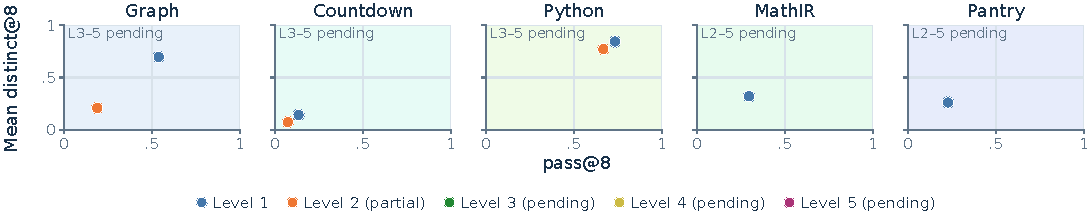
\includegraphics[width=\linewidth]{figures/modebench_level_construction.pdf}
\caption{\textbf{Frozen Qwen2.5-7B at Levels 1--3.}
All 15 cells: level colors, 128 held-out prompts, four $K=8$ groups, $T=1$.
Appendix Figure~\ref{fig:base-levels-all-scales} shows all four scales.}
\label{fig:level-construction}
\end{figure}

\section{ReplayMaxRL: fresh learning with verified memory}
\label{sec:method}\label{sec:maxrl-method}\label{sec:replay}
ReplayMaxRL combines fresh MaxRL updates \citep{tajwar2026maxrl} with
verified-success replay (Figure~\ref{fig:verified-support-story}).

\begin{figure}[!htbp]
\centering
% Crop only blank PDF margins; keep the figure itself unchanged.
\includegraphics[trim={4bp 23bp 4bp 10bp},clip,width=\linewidth]{figures/verified_support_story.pdf}
\caption{\textbf{Fresh MaxRL updates and replay share verified samples.}}
\label{fig:verified-support-story}
\end{figure}

\begin{figure}[!htbp]
\centering
\includegraphics[width=\linewidth]{figures/experiment1_retention_comparator_matrix.pdf}
\caption{\textbf{Replay effects across scales.}
Changes from Dr.GRPO: (A) three scales; (B) Qwen2.5-0.5B alternatives and
initial model. Daggers: four pairs; otherwise five. Averages use shared seeds;
intervals: Appendix~\ref{app:supporting}. Models: \href{https://huggingface.co/od2961/maxent-grpo-models/blob/main/experiments/E78/README.md\#models}{0.5B}, \href{https://huggingface.co/od2961/maxent-grpo-models/blob/main/experiments/E79/README.md\#models}{1B}, \href{https://huggingface.co/od2961/maxent-grpo-models/blob/main/experiments/E80-R1/README.md\#models}{3B}.}
\label{fig:cross-scale-terminal-effects}
\end{figure}

For bank $\mathcal B_x$ with one policy-generated exemplar $e_c$ per admitted
key, replay averages token-normalized log likelihoods:
\begin{equation}
L_{\mathrm{replay}}(x)=-\frac{1}{|\mathcal B_x|}
\sum_{c\in\mathcal B_x}\frac{\log\pi_\theta(e_c\mid x)}{|e_c|}.
\label{eq:lm-verified-replay}
\end{equation}
Equal weights revisit keys independently of discovery frequency. ReplayDr.GRPO
uses Dr.GRPO updates \citep{liu2025understanding}. Conditional categorical theory
shows common-key amplification and fixed-bank protection, without guaranteeing
neural training or sampling visibility (Appendices~\ref{app:theory},~\ref{app:algorithm}).

\section{Does memory preserve verified output support?}
\label{sec:experiments}\label{sec:results}

\begin{figure}[!htbp]
\centering
\includegraphics[width=\linewidth]{figures/e118_all_scale_factorial_progress.pdf}
\caption{\textbf{MaxRL and replay at three model scales.}
Initial--trained--replay tracks average within seed when complete. MaxRL uses
five paired seeds in every domain, including 3B; Falcon Dr.GRPO uses four
common seeds.
\href{https://huggingface.co/od2961/maxent-grpo-models/blob/main/experiments/E118/README.md\#models}{Archived models}.}
\label{fig:maxrl-factorial}
\end{figure}

We measure any-correct probability (\texttt{pass@8}), distinct verified modes
(\texttt{distinct@8}), and their difference, \emph{extra modes}. Breadth depends
on correctness. Correct-key collision $C(q)=\sum_c q_c^2$ rises in all
12 Graph/Pantry baseline comparisons; ReplayDr.GRPO reduces all six.
Joint eligibility and stream reuse limit scope
(Figure~\ref{fig:concentration-story}).

Five seeds train for eight passes. Each domain tests 128 held-out prompts
with four eight-sample groups. Zero-replay-gradient controls share bank code. Figure~\ref{fig:cross-scale-terminal-effects} includes GRPO,
\href{https://huggingface.co/od2961/maxent-grpo-models/blob/main/EXPERIMENTS.md\#direct-comparators}{UCPO} \citep{lochab2026ucpo},
\href{https://huggingface.co/od2961/maxent-grpo-models/blob/main/EXPERIMENTS.md\#direct-comparators}{RLEP-Dr} success replay and
\href{https://huggingface.co/od2961/maxent-grpo-models/blob/main/EXPERIMENTS.md\#semantic-ablations}{semantic entropy}
(protocols: Appendix~\ref{app:experimental-design}).



\noindent\textbf{Replay across scales.}
\label{sec:results-retention}
ReplayDr.GRPO improves both averages at each scale
(Figure~\ref{fig:cross-scale-terminal-effects}).
Uniform key weighting adds $.318$ extra modes over \href{https://huggingface.co/od2961/maxent-grpo-models/blob/main/experiments/E120-R1/README.md\#models}{frequency weighting},
on average at Qwen2.5-0.5B; its correctness contrast is inconclusive
(Figure~\ref{fig:replay-key-weighting}).



\noindent\textbf{Replay beyond MaxRL.}
\label{sec:results-maxrl}
Adding replay improves average correctness and sampled breadth under both
objectives at all three scales (Figure~\ref{fig:maxrl-factorial}).
All 50 Qwen2.5-3B MaxRL endpoints are complete: correctness rises
$.547\to.701$ and modes $.744\to1.107$
(Appendix~\ref{app:maxrl-scale-extensions}; contrasts: Figure~\ref{fig:replay-factorial-effects}).

\begin{figure}[!htbp]
\centering
\includegraphics[width=\linewidth]{figures/modebench_level_admission.pdf}
\caption{\textbf{Replay across difficulty levels: Qwen2.5-0.5B-Instruct.}
Open/filled: Level 1/2. Means equally weight four complete domains within five
paired seeds shared across levels and methods.
Pantry remains separate (Appendix~\ref{app:level2-interim}). \href{https://huggingface.co/od2961/maxent-grpo-models/blob/main/experiments/E119/README.md\#models}{Archived models}.}
\label{fig:level2-admission}
\end{figure}

\noindent\textbf{Harder tasks.}
\label{sec:results-levels}
Four complete five-seed factorials (80/80) show
positive mean replay effects on correctness and sampled breadth within Level 2 (Figure~\ref{fig:level2-admission}); PantryPlan has 10/20 endpoints.
Different test populations prevent an isolated difficulty interpretation
(Figure~\ref{fig:replay-level2-effects}).

\begin{figure}[!htbp]
\centering
\includegraphics[width=\linewidth]{figures/hosted_verified_breadth.pdf}
\caption{\textbf{High accuracy can accompany narrow outputs.}
128 prompts $\times$ eight stateless draws/cell; frozen formatting normalization.
Revised Opus 5 Python wording without a system message prevents a common-prompt
ranking (Appendix~\ref{app:hosted-comparison}).}
\label{fig:hosted-verified-breadth}
\end{figure}

\noindent\textbf{Guidance and draw budget matter.}
In Qwen2.5-0.5B Level-2/3 probes, removing guidance and the Python example
lowers Python correctness (Appendix~\ref{app:prompt-hint-ablation}).
At 64 draws, most trained MathIR conditions remain concentrated; Pantry and
neutral-prompt Python replay reveal alternatives (Appendix~\ref{app:sampling-budget-ablation}).

\noindent\textbf{Hosted concentration.}
\label{sec:hosted-concentration}
Seven deployments often repeat few Graph/MathIR modes despite high accuracy
(Figure~\ref{fig:hosted-verified-breadth}). GPT's 480-prompt no-reasoning sweep
improves pass@8 and breadth from $T=0$ to $1.5$; $T=2$ minus $1.5$ intervals
include zero (Appendix~\ref{app:gpt56-temperature}). Grok's breadth change is inconclusive; Kimi's higher temperature causes
severe truncation (Appendix~\ref{app:hosted-temperature}).

\noindent\textbf{Inference follow-ups.}
Across 32 Pantry problems and two fixed seed pairs, replay raises saved-plan
outage survival by 23.83 points and saves 2.08 recovery calls; correctness also
improves. All 21 hosted 4+4 mixtures beat their average eight-response
constituent in breadth. Coarse factor pairs erase Python's original-wording
Level-3 gain ($.419\to0$), while neutral wording retains $.500$.
Controls, costs and uncertainty: Appendix~\ref{app:inference-followups}.

\noindent\textbf{Conclusion and limits.}
\label{sec:conclusion}\label{sec:discussion}\label{sec:limitations}
Fixed-bank scores retain a declining tail (Appendix~\ref{app:fixed-bank-survival}).
Exact mode probabilities and causal accuracy mechanisms remain unverified.

\label{main:lastpage}

\clearpage
\bibliographystyle{plainnat}
\bibliography{example_paper}
\clearpage
\appendix
% Reorganized supplement; the root supplies the appendix counter.
\raggedbottom
\section*{Supplementary Material}
\label{app:organization}
The supplement opens with the claim--evidence map
(Appendix~\ref{app:claim-basis}), then gives measurement identities and the
complete conditional theory (Appendices~\ref{app:metric-details} and~\ref{app:theory}).
Benchmark construction, full prompts, and the implemented algorithm follow.
Controlled results (Appendix~\ref{app:supporting}) precede longitudinal
diagnostics (Appendix~\ref{app:ablations}) and the separate hosted observations.
Prompt interventions and reproducibility close the scientific record.
All original proof statements and proofs are retained; detailed figures now
sit beside the claims and controls they support.

\long\def\crossscaletablematerial{%

\begin{table}[H]
  \centering
  \caption{\textbf{Matched results after eight training passes.} Columns compare Dr.GRPO with ReplayDr.GRPO after exactly eight training passes. Entries are means over the displayed paired-seed intersection;
  $n$@pass gives its size and training pass. P, M, and D denote
  \texttt{pass@8}, \texttt{mean@8}, and \texttt{distinct@8}. Every available
  source-admissible terminal pair is included, no shallower checkpoint is carried forward, and
  no missing result is imputed. Falcon Countdown uses four admissible seeds
  (Appendix~\ref{app:source-integrity}). Pale green marks a ReplayDr.GRPO mean that is
  strictly higher than its matched Dr.GRPO mean. Archived models: \href{https://huggingface.co/od2961/maxent-grpo-models/blob/main/experiments/E78/README.md\#models}{Qwen2.5-0.5B}, \href{https://huggingface.co/od2961/maxent-grpo-models/blob/main/experiments/E79/README.md\#models}{Falcon3-1B}, and \href{https://huggingface.co/od2961/maxent-grpo-models/blob/main/experiments/E80-R1/README.md\#models}{Qwen2.5-3B}.}
  \label{tab:core-terminal-endpoints}
  \scriptsize
  \setlength{\tabcolsep}{3.2pt}
  \resizebox{\linewidth}{!}{%
  \begin{tabular}{@{}llc*{6}{r}@{}}
    \toprule
    \textbf{Model} & \textbf{Domain} & \textbf{$n$@pass} &
      \multicolumn{3}{c}{\textbf{Dr.GRPO}} &
      \multicolumn{3}{c}{\textbf{ReplayDr.GRPO}} \\
    \cmidrule(lr){4-6}\cmidrule(l){7-9}
      & & & \textbf{P} & \textbf{M} & \textbf{D}
      & \textbf{P} & \textbf{M} & \textbf{D} \\
    \midrule
    \input{results/core_terminal_endpoints_table_body.tex}
  \end{tabular}}
\end{table}

}


\section{Claims and Their Evidential Basis}
\label{app:claim-basis}

The training and hosted studies share a measurement question: how is correct
probability allocated among verified alternatives? They supply different
kinds of evidence. The table states the basis of each central claim and the
inference it supports; motivating downstream benefits remain hypotheses.

\begin{table}[H]
\centering
\small
\setlength{\tabcolsep}{5pt}
\renewcommand{\arraystretch}{1.16}
\begin{tabularx}{\linewidth}{@{}p{.21\linewidth}p{.22\linewidth}X@{}}
\toprule
\textbf{Claim} & \textbf{Identifiable basis} & \textbf{Scope of the inference} \\
\midrule
Success and breadth differ & Identity and concavity: Lemma~\ref{lem:success-breadth} &
At fixed correctness, concentration in majorization order lowers expected breadth.
More correct samples can also raise the raw mode count. \\
Uniform categorical replay balances mass & Identity: Equation~\eqref{eq:replay-bank-decomposition} &
Likelihood replay already contains a balancing term. This neither requires a
separate balance loss nor equates exemplar scores with key probabilities. \\
Binary reward can induce collapse & Conditional theorem: Theorem~\ref{thm:grpo-collapse} &
Independent canonical-outcome logits, common length normalization, Euclidean
mean flow, and a unique initial winner; no neural-optimizer guarantee. \\
Replay remains available when fresh gradients vanish & Conditional score calculation:
Appendix~\ref{app:theory-gradient-availability} &
Equal-reward groups have zero centered task update; bank scoring need not.
An available gradient does not ensure improvement after a shared-parameter update. \\
Persistent replay protects banked modes & Conditional theorem and corollary:
Theorem~\ref{thm:replay-retention}, Corollary~\ref{cor:replay-no-collapse} &
Fixed bank, fixed positive dose, and the stated mean flow yield probability
floors. Uniformity needs full coverage and equal categorical weights;
unbanked modes may vanish. \\
Exemplar loss can bound key probability & Conditional lemma:
Lemma~\ref{lem:shared-exemplar-retention} &
A bounded joint potential and complete-response likelihood under the same
sampling law protect those prompts. Neither held-out transfer nor visibility
in eight draws follows. \\
Training can concentrate correct-key outputs & Retrospective longitudinal comparison:
Appendix~\ref{app:conditional-concentration} &
Graph/Pantry Dr.GRPO and GRPO show increased collision at each scale.
Eligibility and stream sensitivities limit the observed population; exact
support extinction is not identified. \\
Replay can reduce conditional concentration & Retrospective matched replay comparison:
Appendix~\ref{app:conditional-concentration} &
ReplayDr.GRPO reduces collision in Graph/Pantry at each scale. Correctness
can also change on those eligible prompts; this is not an all-prompt effect. \\
Replay improves measured endpoints & Controlled comparisons:
Figure~\ref{fig:replay-factorial-effects} &
Paired replay additions isolate the implemented intervention within the
reported model/domain cohorts. All five 3B MaxRL blocks use five paired
seeds; individual-mode retention is not identified. \\
Equal key weights can aid breadth & Controlled weighting comparison:
Appendix~\ref{app:frequency-replay-progress} &
Uniform versus fresh-frequency weighting changes extra sampled modes in the
reported cohorts; the average correctness contrast is inconclusive. \\
Replay can help on Level 2 & Controlled within-level comparisons:
Figure~\ref{fig:replay-level2-effects} &
Four complete domains support within-level replay effects. Separate terminal
test splits prevent a pure cross-level difficulty-effect interpretation. \\
Fixed exemplars show heterogeneous score changes & Exploratory longitudinal finding:
Appendix~\ref{app:fixed-bank-survival} &
Central scores improve while a tail declines. No matched no-replay bank arm
identifies a causal retention effect or exact key probabilities. \\
Accurate hosted outputs can be concentrated & Exploratory deployment comparison:
Appendix~\ref{app:hosted-comparison} &
Observed correctness and breadth describe the stated protocols. They do not
identify RLVR as the cause, a model-size effect, or training-time collapse. \\
Temperature changes observed breadth & Exploratory matched-prompt comparison:
Appendix~\ref{app:gpt56-temperature} &
Four temperature settings describe one deployment and reasoning profile.
The best observed point does not establish an optimal sampling temperature in general. \\
\bottomrule
\end{tabularx}
\caption{\textbf{What each central claim rests on.} Identities concern the
sampling law, theorems specify conditional dynamics, and experiments support
the stated intervention or exploratory observation. All reported intervals
are nominal and unadjusted.}
\label{tab:claim-basis}
\end{table}

The before/after verifier-training precheck is a longitudinal checkpoint
comparison (Appendix~\ref{app:pre-rl-regression}). Its extra-mode declines
are measured changes in the registered runs, not proof of zero probability
for lost keys or a universal decrease in raw breadth across domains.

\section{Formal Metric Definitions}
\label{app:metrics}
\label{app:metric-details}
\label{sec:collapse-metrics}

For prompt $x$ with specification $s_x$, the validator maps an output to a
canonical valid key or failure:
$V(\cdot,s_x):\mathcal Y\to\mathcal C_x\cup\{\bot\}$.
The learner sees keys only for its generated responses, never the full
catalogue $\mathcal C_x$ or its size. For $Y\sim\pi_\theta(\cdot\mid x)$, define
\[
 P_\theta^+(x)=\Pr[V(Y,s_x)\ne\bot],\qquad
 p_\theta^+(c\mid x)=\Pr[V(Y,s_x)=c\mid V(Y,s_x)\ne\bot].
\]
The conditional distribution is defined only when $P_\theta^+(x)>0$;
otherwise all sampling metrics below are zero. Mode collapse means
concentration onto fewer valid keys, which can coexist with increasing
success probability.

For $K$ independent responses, let
\[
 D_K=\bigl|\{V(Y_i,s_x):i\le K\}\setminus\{\bot\}\bigr|,
 \qquad F_K=K^{-1}\sum_i\1[V(Y_i,s_x)\ne\bot].
\]
Then \texttt{distinct@}$K=\E[D_K]$ counts expected unique verified keys in
$[0,K]$, whereas \texttt{pass@}$K=\Pr[D_K>0]$ and
\texttt{mean@}$K=\E[F_K]$ are probabilities in $[0,1]$.
The samplewise inequality $F_K\le\1[D_K>0]\le D_K$ gives
$\texttt{mean@}K\le\texttt{pass@}K\le\texttt{distinct@}K$,
but changes in the count and probability have different units.
\begin{lemma}[Success and sampled breadth]
\label{lem:success-breadth}
Fix a prompt, a finite or countable valid-key set, and $K\ge1$ independent
draws from the same fixed sampling law. Let
$\mu_c=\Pr[V(Y,s_x)=c]$ and $P=\sum_c\mu_c$. Then
\begin{equation}
 S_K:=\texttt{pass@}K=1-(1-P)^K,\qquad
 B_K:=\texttt{distinct@}K=\sum_c[1-(1-\mu_c)^K].
 \label{eq:success-breadth-identities}
\end{equation}
For a finite valid-key set of size $m\ge1$ and $P>0$, write $q_c=\mu_c/P$.
At fixed $P$, $B_K$ is Schur-concave in $q$: if $q$ majorizes $q'$
(its decreasingly sorted partial sums are at least those of $q'$), then
$B_K(P,q)\le B_K(P,q')$. In particular,
\begin{equation}
 1-(1-P)^K\le B_K(P,q)\le m[1-(1-P/m)^K].
 \label{eq:fixed-success-breadth-bounds}
\end{equation}
For $K\ge2$, the lower bound is attained only by concentration on one key,
and the upper bound only by uniform $q$. For $K=1$, $B_1=P$ for every $q$.
At fixed $q$, increasing $P$ cannot decrease $B_K$.
\end{lemma}
\begin{proof}
All $K$ draws fail with probability $(1-P)^K$. For each key $c$, its
appearance indicator has expectation $1-(1-\mu_c)^K$; summing indicators
gives the second identity, also for countably many keys by nonnegativity.
For fixed $P>0$ and $K\ge2$, the function
$f(v)=1-(1-Pv)^K$ is strictly concave on $[0,1]$.
Transferring mass from a larger coordinate to a smaller one without reversing
their order increases $\sum_c f(q_c)$; successive such transfers give the
majorization assertion. The point mass and uniform vector are its extreme
cases, giving the bounds and equality conditions. Finally,
$\partial B_K/\partial P=K\sum_c q_c(1-Pq_c)^{K-1}\ge0$,
which proves monotonicity in correctness.
\end{proof}

These are promptwise identities, before averaging over prompts. In particular,
applying the nonlinear formula to a mean correctness generally changes the
result. They explain the shared measurement in the training and hosted
studies: success depends on total correct mass; sampled breadth also depends
on its allocation. More breadth alone proves neither greater conditional
diversity nor better success, and neither metric establishes downstream utility.

Raw
\texttt{distinct@}$K$ measures sampled coverage, not total
positive-probability support. Uniform independent sampling from $N$ finite
actions, with $n_c$ aliases of valid key $c$, gives
$\sum_c[1-(1-n_c/N)^K]$ expected keys; open-ended program spaces have no
canonical uniform generator.

The terminal co-primary outcomes use $K=8$: success probability
\texttt{pass@8} and raw \texttt{distinct@8}. Their difference
$\E[D_K-\1[D_K>0]]$ counts extra verified modes beyond the first. This
interpretive decomposition remains coupled to correctness and is neither
a third primary endpoint nor a success-matched diversity measure.

\subsection{Why balance within the replay bank}
\label{app:replay-metric-alignment}

Uniform sampling over keys prevents discovery frequency from determining replay
frequency. To explain its relationship to the evaluation metric, we first
analyze an equal-weight categorical surrogate, without length normalization.
A stored response's probability need not equal its key's total probability.
For $C=|\mathcal B_x|$ banked keys, write $p(c)$ for their probabilities
and $q_{\mathcal B}$ for their total mass. Then
\begin{equation}
 -\frac1C\sum_{c\in\mathcal B_x}\log p(c)
 =-\log q_{\mathcal B}+\log C+
   \mathrm{KL}\!\left(U_C\,\|\,
   p(c\mid c\in\mathcal B_x)\right).
 \label{eq:replay-bank-decomposition}
\end{equation}
The objective rewards greater banked verified mass and a more balanced
conditional distribution, aligning with \texttt{pass@}$K$ and
\texttt{distinct@}$K$. The combined update need not improve both at every step. Indeed banked-key coverage contributes
$\sum_c[1-(1-p(c))^K]$ to expected \texttt{distinct@}$K$; at fixed
$q_{\mathcal B}$ and $C$, concavity makes it largest under uniform allocation,
while $1-(1-q_{\mathcal B})^K$, the probability of any banked key, depends
only on total mass. This deliberate objective--metric alignment motivates
treating held-out \texttt{pass@}$K$ as co-primary. Uniformity also maximizes the
smallest conditional banked-key mass, making equal retention explicit. Banks
contain only training-prompt responses; evaluation responses never enter
training.




% Shared long-paper and workshop benchmark/protocol appendix.

\section{Mode Collapse and Verified Replay}
\label{app:theory}

Under the explicit categorical assumptions below, centered binary-reward
estimators amplify a pre-existing imbalance among correct modes,
whereas persistent verified replay supplies a loss barrier for banked modes.
The complete-response argument then states what would be needed to transfer
that protection to a language model. These results concern idealized update
rules; they do not certify the implemented AdamW/PPO trajectories.

\subsection{Categorical abstraction and mean updates}
\label{app:theory-grpo-mean}

Fix one isolated prompt and a finite category set
$\mathcal A=\mathcal C\mathbin{\dot\cup}\mathcal N$, with $m\ge2$ correct
execution modes and $n\ge1$ incorrect categories. Assign one independently
optimized logit to each category, including one logit per canonical correct
mode, and set $p_a=\operatorname{softmax}(z)_a$,
$P=\sum_{c\in\mathcal C}p_c$, and $q_c=p_c/P$. Thus $P$ measures correctness
and $q$ the conditional distribution among correct modes. Logits are finite
initially, $0<P(0)<1$, and explicit reference KL is zero. The collapse result
uses Euclidean infinitesimal expected updates in these logits, without
optimizer preconditioning, momentum, or another regularizer.

A language model induces probabilities over canonical outcomes, but this
identification of probabilities does not identify its update geometry.
Aggregating several response strings into a mode does not generally commute
with gradient flow in response logits. One independent logit per canonical
outcome is therefore an explicit abstraction, not a reduction proved for the
neural policy or its validator equivalence classes.

Draw a group $A_1,\ldots,A_G\stackrel{\mathrm{iid}}{\sim}p$ with $G\ge2$,
write $R_i=\1[A_i\in\mathcal C]$, and let $M=\sum_iR_i$. At the on-policy
point where the PPO ratio equals one, consider the common-length estimator
\begin{equation}
  \widehat g_G
  =\frac1G\sum_{i=1}^G
   w(M)\left(R_i-\frac{M}{G}\right)\nabla_z\log p_{A_i}.
  \label{eq:group-estimator}
\end{equation}
For the Dr.GRPO abstraction, $w(M)=1$ after absorbing the shared positive
length scale. Reward-standardized GRPO with equal or common response-length
normalization takes $w(M)$ to be the reciprocal group reward standard
deviation on mixed groups (with a fixed numerical stabilizer if used).
Standard variable-length GRPO also weights each response by its own inverse
length \citep{shao2024deepseekmath,liu2025understanding}; that factor cannot
generally be absorbed into $w(M)$ and is outside the equivalence proved here.
In either included case, $0<w(\ell)<\infty$ for
$\ell\in\{1,\ldots,G-1\}$. We define the entire update as zero on all-equal
groups without evaluating an undefined reciprocal standard deviation;
likewise, $w(M)M(G-M)$ below is defined as zero when $M=0$ or $M=G$. All
advantages and normalization weights are detached in the score estimator.

\begin{lemma}[A group baseline does not remove frequency amplification]
\label{lem:grpo-mean}
For $0<P<1$, the expected update in Equation~\eqref{eq:group-estimator} is
\begin{equation}
  \E[\widehat g_G]
  =c_G(P)\nabla_z P,
  \qquad
  c_G(P)=
  \frac{\E\!\big[w(M)M(G-M)\big]}{G^2P(1-P)}>0.
  \label{eq:expected-group-gradient}
\end{equation}
For the Dr.GRPO abstraction, $c_G(P)=(G-1)/G$. Group centering and reward
standardization rescale the expected gradient without changing its direction
under these assumptions.
\end{lemma}

\begin{proof}
Condition on the complete binary reward vector, whose sum is $M$. The score
identities give
\[
  \E[\nabla_z\log p_{A_i}\mid R_i=1]=\nabla_z\log P,
  \qquad
  \E[\nabla_z\log p_{A_i}\mid R_i=0]
  =\nabla_z\log(1-P).
\]
There are $M$ correct rows with centered reward $(G-M)/G$ and $G-M$
incorrect rows with centered reward $-M/G$. Therefore the conditional
expectation of the unaveraged sum in~\eqref{eq:group-estimator} is
\[
  w(M)\frac{M(G-M)}{G}
  \left(\nabla_z\log P-\nabla_z\log(1-P)\right)
  =w(M)\frac{M(G-M)}{GP(1-P)}\nabla_zP.
\]
The outer factor $1/G$ and expectation over
$M\sim\operatorname{Binomial}(G,P)$ yield~\eqref{eq:expected-group-gradient}.
For $w\equiv1$,
$\E[M(G-M)]=G(G-1)P(1-P)$, proving the Dr.GRPO value.
\end{proof}

The binomial identity also gives the denominator-free expression
\[
 c_G(P)=\frac{G-1}{G}\sum_{j=0}^{G-2}\binom{G-2}{j}
 w(j+1)P^j(1-P)^{G-2-j}.
\]
The binomial weights sum to one, so $c_G$ lies between
$(G-1)\min_j w(j+1)/G$ and $(G-1)\max_j w(j+1)/G$.
This establishes the smooth, positive extension to $P=0,1$ used in the
subsequent flow and convergence arguments.

The next lemma specializes the practical-estimator analysis of
\citet[Section~4.3 and Appendix~D, Theorem~5]{tajwar2026maxrl}
to our categorical notation; we include the derivation for completeness.

\begin{lemma}[Binary MaxRL has the same correctness-gradient direction]
\label{lem:maxrl-mean}
Under the same categorical and common-length assumptions, let MaxRL assign
$A_i^{\mathrm{MaxRL}}=GR_i/M-1$ when $M>0$ and zero when $M=0$, as in
Section~\ref{sec:maxrl-method}. For
$\widehat g_G^{\mathrm{MaxRL}}=G^{-1}\sum_i
 A_i^{\mathrm{MaxRL}}\nabla_z\log p_{A_i}$ at the on-policy point, the
expected update is
\begin{equation}
  \E[\widehat g_G^{\mathrm{MaxRL}}]
  =c_G^{\mathrm{MaxRL}}(P)\nabla_zP,
  \qquad
  c_G^{\mathrm{MaxRL}}(P)
  =\frac{1-(1-P)^{G-1}}{P}>0,
  \label{eq:maxrl-expected-gradient}
\end{equation}
with continuous endpoint values
$c_G^{\mathrm{MaxRL}}(0)=G-1$ and
$c_G^{\mathrm{MaxRL}}(1)=1$.
\end{lemma}

\begin{proof}
Condition on $M=m>0$. Each successful row has advantage $(G-m)/m$ and each
failed row has advantage $-1$. Using the same conditional score identities as
above, the expected unaveraged sum is
\[
  (G-m)\!\left(\nabla_z\log P-\nabla_z\log(1-P)\right)
  =\frac{G-m}{P(1-P)}\nabla_zP.
\]
After the outer factor $1/G$ and averaging over
$M\sim\operatorname{Binomial}(G,P)$,
\[
 \E[(G-M)\1\{M>0\}]
 =G(1-P)-G\Pr(M=0)
 =G\big[(1-P)-(1-P)^G\big].
\]
Substitution gives Equation~\eqref{eq:maxrl-expected-gradient}. Its endpoint
values follow by continuity (or the finite geometric-series identity), which
also gives the stated continuous extension at both boundaries.
\end{proof}

The same finite-series identity gives the potential used below:
\begin{equation}
 \Psi_{\mathrm{MaxRL}}(P)
 :=\int_0^P c_G^{\mathrm{MaxRL}}(s)\,ds
 =\sum_{k=1}^{G-1}\frac{1-(1-P)^k}{k}.
 \label{eq:maxrl-potential-finite-sum}
\end{equation}
In particular, $\Psi_{\mathrm{MaxRL}}(1)=\sum_{k=1}^{G-1}1/k$.
For binary rewards, best@\(k\) equals pass@\(k\), so this is a harmonic
mixture of sampling objectives for $k=1,\ldots,G-1$. The upper limit is
$G-1$, not $G$: the implemented centered estimator drops the entire update
on all-failure groups. Subtracting an unconditional score baseline even on
those groups instead gives the order-$G$ estimator. This distinction concerns
the exact finite-group expectation at the on-policy point; it does not assert
unbiasedness of subsequent clipped or adaptive-optimizer updates.


\subsection{Winner-take-all collapse in the categorical mean flow}
\label{app:theory-collapse}

Consider $\dot z=c_G(P)\nabla_zP$, with any of the smooth positive
coefficients established above: Dr.GRPO, common-length reward-standardized
GRPO, or the specified centered binary MaxRL estimator. This infinitesimal
expected-update model removes
sampling noise and retains independently trained Euclidean logits. The
conditional dynamics reduce to the standard frequency-dependent replicator
system with fitness $f_c(q)=q_c$ \citep{hofbauer1998evolutionary}. The result is
a specialization to the group estimators, not a new general theorem about
replicator dynamics. Related correctness-indifferent collapse analyses include
\citet{sinha2026expected,lochab2026ucpo}.

\begin{theorem}[Standard replicator specialization for binary-reward RL]
\label{thm:grpo-collapse}
Under the independent-logit mean-flow assumptions above, start from finite
logits with $0<P(0)<1$. If the conditional correct-mode
distribution $q(0)$ has a unique largest coordinate $c^\star$, then
\[
  P(t)\longrightarrow1,
  \qquad
  q_{c^\star}(t)\longrightarrow1,
  \qquad
  q_c(t)\longrightarrow0\quad(c\ne c^\star).
\]
Thus these categorical mean flows converge to a single correct execution
mode for generic initial conditions, even though every mode in $\mathcal C$
has exactly the same reward. This is an asymptotic statement within the
specified update geometry, not a claim of finite-time support loss or a
convergence guarantee for the stochastic neural optimizers used in our experiments.
\end{theorem}

\begin{proof}
The coefficient $c_G$ is smooth and bounded on $[0,1]$, and the softmax
reward gradient is bounded. Thus the logit flow exists for all finite times
and cannot develop infinite logits at finite time.
For a correct mode $c$ and incorrect category $a$,
\[
  \dot z_c=c_G(P)p_c(1-P),
  \qquad
  \dot z_a=-c_G(P)p_aP.
\]
Also $\dot P=c_G(P)\lVert\nabla_zP\rVert_2^2>0$. If $P$ converged to an
interior value, continuity and positivity of $c_G$, together with
\[
 \lVert\nabla_zP\rVert_2^2
 \ge P^2(1-P)^2\left(\frac1m+\frac1n\right),
\]
would keep $\dot P$ bounded away from zero, a contradiction. Hence $P\to1$.

Define the effective optimization time
\[
  \tau(t)=\int_0^t c_G(P(s))P(s)(1-P(s))\,ds.
\]
If $\tau(\infty)<\infty$, every correct and incorrect logit would have finite
total variation, because the absolute velocity of each is at most $\dot\tau$.
All logits would then converge to finite values, contradicting $P\to1$.
Therefore $\tau(t)\to\infty$, leaving infinite effective time for the
correct-simplex dynamics below.

On the correct simplex, changing from $t$ to $\tau$ gives the replicator flow
\begin{equation}
  \frac{dq_c}{d\tau}
  =q_c\left(q_c-\sum_{d\in\mathcal C}q_d^2\right),
  \qquad
  \frac{d}{d\tau}\log\frac{q_c}{q_d}=q_c-q_d.
  \label{eq:grpo-replicator}
\end{equation}
The initially unique maximum remains the unique maximum. For $c\ne c^\star$,
set $\xi_c=q_c/q_{c^\star}$, so $\xi_c(0)<1$ and $\xi_c$ is nonincreasing.
Since $q_{c^\star}\ge1/m$,
\[
 \frac{d\log\xi_c}{d\tau}
 =-q_{c^\star}(1-\xi_c)
 \le-\frac{1-\xi_c(0)}{m}.
\]
Hence $\xi_c(\tau)\le\xi_c(0)\exp[-(1-\xi_c(0))\tau/m]\to0$.
Every competing mode vanishes relative to $c^\star$; normalization then
yields $q_{c^\star}\to1$, establishing the claimed single-mode limit.
\end{proof}

If several modes tie for the largest initial probability, symmetry preserves
the tie; the same ratio argument eliminates strictly smaller coordinates and
leaves the tied maxima uniform. An exactly uniform correct distribution is
therefore a special initial condition. The theorem concerns limiting
concentration: finite softmax logits already give positive probabilities at
every finite time, so finite-time positivity alone is not a retention result.

\paragraph{Dependence on optimization geometry.}
For a smooth parameterization $z=z(\theta)$ with Jacobian
$J_\theta=\partial z/\partial\theta$, Euclidean parameter flow instead
induces $\dot z=c_G(P)J_\theta J_\theta^\top\nabla_zP$. The independently
trained logit theorem uses $J_\theta J_\theta^\top=I$ and does not automatically
extend to arbitrary shared parameters or another optimization metric. Equal
binary reward alone does not force this winner selection: the categorical
natural-gradient reward flow can be represented by
$\dot z_a=c_G(P)(R_a-P)$, which gives identical velocities to correct logits
and preserves their ratios. Here $R_a=\1[a\in\mathcal C]$.
Parameter count alone does not specify the optimization geometry. The empirical
scale
comparisons also change pretrained models and learning-rate schedules; they
neither measure the geometry nor identify the cause of cross-scale differences.
The theorem supplies a mechanism to test in controlled training; it cannot
identify the training history or cause of concentration in a hosted model.

\subsection{A replay signal when fresh groups supply none}
\label{app:theory-gradient-availability}

\begin{lemma}[Fresh-group starvation and replay signal]
\label{lem:replay-gradient-availability}
Fix the categorical policy above with correctness probability $P$, and draw
$G\ge2$ fresh categories independently. The probability of a mixed-reward
group is
\[
 h_G(P)=1-P^G-(1-P)^G\le G\min\{P,1-P\}.
\]
Every all-equal group has zero fresh task component for
Equation~\eqref{eq:group-estimator} and the specified centered MaxRL
estimator. A nonzero fresh task component therefore requires a mixed group,
so its probability is at most $h_G$. This gives no lower bound on gradient
magnitude and says nothing about other loss terms, clipping, or an optimizer step carrying momentum across successive updates.

For a nonempty fixed verified bank $\mathcal B\subseteq\mathcal C$ with
normalized positive weights $w_b$, let
$R_w=-\sum_b w_b\log p_b$ and $\rho_w>0$. Extend $w$ by zero outside the
bank to obtain $\bar w$. The deterministic replay ascent vector is
\[
 v^{\rm replay}=-\rho_w\nabla R_w=\rho_w(\bar w-p),
\]
which vanishes only at $p=\bar w$. In particular, if $p_b\le w_b/2$ for a banked
mode, then $v^{\rm replay}_b\ge\rho_w w_b/2$, even when $b$ is absent from the
fresh group. For a uniform bank of $k\ge2$ modes and fixed $\rho_w>0$, as
$p\to\mathbf e_b$ at one banked correct mode, $h_G(P)\to0$ whereas
$\|v^{\rm replay}\|_2\to\rho_w\sqrt{1-1/k}>0$.
The replay norm therefore stays positive as fresh task-signal opportunities vanish.
\end{lemma}

\begin{proof}
The all-correct and all-incorrect events are disjoint and have probabilities
$P^G$ and $(1-P)^G$. A mixed group requires both a correct and an incorrect
sample; the union bound gives the two bounds $GP$ and $G(1-P)$.
For $R_w=-\sum_b w_b\log p_b$, the softmax score identity gives
$\partial R_w/\partial z_a=p_a-\bar w_a$, proving the replay formula and
coordinate bound. Finally,
\[
 \|\bar w-\mathbf e_b\|_2^2=(1-1/k)^2+(k-1)/k^2=1-1/k,
\]
which gives the strictly positive limiting norm for $k\ge2$.
\end{proof}


The displayed replay vector averages the fixed bank. A stochastic exemplar
draw has this vector only in expectation, and a nonzero logit coordinate can
be annihilated by a degenerate neural Jacobian. Replay also need not increase
the next mixed-group probability: $h_G(P)$ is largest at $P=1/2$. The claim
is that a banked target can supply a separate verified signal when the fresh
task gradient is unavailable.

A bounded advantage based on fresh samples has a different boundary behavior.
The next bound includes group-dependent detached scores and distinguishes
sampled updates from gradients of an exactly evaluated entropy functional.

\begin{lemma}[Bounded sampled scores have no probability-independent boundary force]
\label{lem:sampled-score-bound}
In the same independent-logit model, condition on the training history, draw
$A_1,\ldots,A_G$ independently from $p$, and let $a_i$ be any detached,
possibly group-dependent advantages with $|a_i|\le B$. To interpret the
bound uniformly as $p_b\to0$, assume a finite $B$ independent of that limit.
At the on-policy point define
\[
 \widehat g=\frac1G\sum_{i=1}^G a_i(\mathbf e_{A_i}-p).
\]
For every category $b$,
\[
 |\E[\widehat g_b]|\le\E|\widehat g_b|
 \le 2B p_b(1-p_b).
\]
On a group with no draw of $b$, exactly
$\widehat g_b=-p_bG^{-1}\sum_i a_i$; it is zero if the applied advantages
sum to zero. By comparison, the verified-replay component for a fixed target
$w$ has logit velocity $\rho(w_b-p_b)$, which approaches $\rho w_b>0$
for a banked category as $p_b\to0$.
\end{lemma}

\begin{proof}
Use the triangle inequality and $|a_i|\le B$. Each marginal draw satisfies
$\E|\1\{A_i=b\}-p_b|=2p_b(1-p_b)$, irrespective of the dependence of
$a_i$ on the group. On the absence event all indicator terms are zero.
The replay formula follows by differentiating $-\sum_b w_b\log p_b$.
\end{proof}

The bound compares the isolated logit-gradient components. It does not prove
inevitable collapse, rule out retention by a bounded estimator, or guarantee
that replay dominates the full update. An unsampled mode can still change
through softmax normalization or shared parameters. Exact entropy is outside
the uniformly bounded-score premise because its surprisal is unbounded near
zero; the lemma is not an impossibility result for entropy regularization.
Nor does the absence of a mode from a finite sample establish zero probability.


\subsection{Fixed-bank replay and qualitative retention}
\label{app:theory-replay}

Let $\mathcal B\subseteq\mathcal C$ be a nonempty fixed bank of $k$ modes that
the policy has produced and the validator has accepted. Uniform verified replay
uses one exemplar per banked mode and, in the categorical reduction, minimizes
\begin{equation}
  R_{\mathcal B}(z)
  =-\frac1k\sum_{b\in\mathcal B}\log p_b.
  \label{eq:verified-replay-loss}
\end{equation}
This is ordinary cross-entropy against the distribution that assigns mass
$1/k$ to each banked mode and zero elsewhere. It is not conditioned on the
bank: decreasing~\eqref{eq:verified-replay-loss} can raise total bank mass as
well as redistribute mass within the bank.

In an averaged continuous-time model, absorb a fixed round-robin replay
frequency and loss scale into an effective dose $\rho>0$. This assumes a
fixed eligible-bank set and constant relative weighting; it does not identify
finite alternating updates with simultaneous gradient flow. The prompt-isolated categorical mean flow for any of the three fresh
binary-reward objectives above plus verified replay is
\begin{equation}
  \dot z
  =c_G(P)\nabla_zP-\rho\nabla_zR_{\mathcal B}(z).
  \label{eq:replay-mean-flow}
\end{equation}
Let $\Psi(P)=\int_0^P c_G(s)\,ds$. For the finite-group estimators in Lemmas~\ref{lem:grpo-mean}
and~\ref{lem:maxrl-mean}, $c_G$ has a finite positive extension to $[0,1]$;
in particular, Dr.GRPO has $c_G=(G-1)/G$ and MaxRL has
$c_G=[1-(1-P)^{G-1}]/P$. Define
\begin{equation}
  F_{\mathcal B}(z)=\rho R_{\mathcal B}(z)-\Psi(P(z)).
  \label{eq:replay-potential}
\end{equation}
Then~\eqref{eq:replay-mean-flow} is exactly gradient flow
$\dot z=-\nabla_zF_{\mathcal B}$.

\begin{theorem}[Verified replay prevents banked-mode extinction]
\label{thm:replay-retention}
Suppose logits are finite at time $T$ and thereafter the nonempty verified
bank $\mathcal B$ is fixed, fits within replay capacity, and receives a
fixed positive effective replay dose $\rho$. Under~\eqref{eq:replay-mean-flow}, define
\[
  C_T
  =R_{\mathcal B}(z(T))
   +\frac{\Psi(1)-\Psi(P(T))}{\rho}.
\]
Then for every $b\in\mathcal B$ and every $t\ge T$,
\begin{equation}
  p_b(t)\ge \exp(-kC_T)>0.
  \label{eq:replay-retention-bound}
\end{equation}
Thus each banked probability is uniformly bounded away from zero for all
$t\ge T$, including asymptotically, even when the bank does not cover every
correct mode. This is stronger than finite-time positivity, which already
follows from finite softmax logits without replay.
\end{theorem}

\begin{proof}
The smooth vector field has bounded velocity because $c_G$,
$\nabla_zP$, and $\nabla_zR_{\mathcal B}$ are bounded, so finite initial
logits give a flow for every finite $t\ge T$. Along this flow,
\[
  \frac{d}{dt}F_{\mathcal B}(z(t))
  =-\lVert\nabla_zF_{\mathcal B}(z(t))\rVert_2^2\le0.
\]
Since $P(t)\le1$ and $\Psi$ is increasing,
\[
  R_{\mathcal B}(z(t))
  \le R_{\mathcal B}(z(T))
     +\frac{\Psi(1)-\Psi(P(T))}{\rho}
  =C_T.
\]
Every $-\log p_b$ is nonnegative and their sum is
$kR_{\mathcal B}$. Therefore
$-\log p_b(t)\le kC_T$ for every banked mode, which is exactly
Equation~\eqref{eq:replay-retention-bound} for every time after $T$.
\end{proof}


The floor is qualitative and can be numerically vacuous. For example, at
$k=16$ even a hypothetical $C_T=160$ gives $e^{-2560}$, far below any useful
evaluation probability. The argument establishes a uniform-in-time lower
bound in the stated ideal flow, not practical visibility or a prediction for
the experimental replay loss. The effective dose also depends on relative
fresh/replay frequencies, not the replay coefficient alone.

A common nonnegative, locally integrable rate $\eta(t)$ multiplying both
terms of~\eqref{eq:replay-mean-flow} preserves the energy bound, since
$\dot F_{\mathcal B}=-\eta(t)\|\nabla F_{\mathcal B}\|_2^2\le0$.
The convergence statements below additionally require
$\int_T^\infty\eta(t)\,dt=\infty$ and then follow by reparameterizing
optimization time. Infinitely many replay visits alone establish neither
this condition nor a fixed replay-to-fresh weighting. Different time-varying
relative weights are outside the fixed-potential argument.

\paragraph{Full coverage and the categorical target.}
\begin{corollary}[Conditional full-coverage categorical limit]
\label{cor:replay-no-collapse}
Assume the conditions of Theorem~\ref{thm:replay-retention} and that by time
$T$ the bank covers the full correct support, $\mathcal B=\mathcal C$. Let
$u_c=1/m$ on $\mathcal C$. Then the categorical mean flow converges to
\[
  P(t)\longrightarrow1,
  \qquad q(t)\longrightarrow u.
\]
Consequently
\[
  \min_{c\in\mathcal C}q_c(t)\longrightarrow\frac1m,
  \qquad
  \mathcal H(q(t))\longrightarrow\log m,
\]
and conditional correct-mode collapse is impossible.
\end{corollary}

\begin{proof}
For full coverage,
\begin{equation}
 R_{\mathcal C}=\log m-\log P+\mathrm{KL}(u\|q).
 \label{eq:replay-mass-uniformity-decomposition}
\end{equation}
The potential is bounded below by $-\Psi(1)$, so its descent gives
$\int_T^\infty\|\nabla F_{\mathcal C}\|_2^2dt<\infty$. The finite-group
$c_G$ is smooth on $[0,1]$, and softmax derivatives and the cross-entropy
gradient are bounded. Thus the Hessian of $F_{\mathcal C}$ and the velocity
are bounded; the gradient along the trajectory is uniformly continuous.
Square integrability then implies $\nabla F_{\mathcal C}\to0$: recurring
gradients of fixed positive size would otherwise contribute energy over
intervals of a uniform minimum length.

Every limiting probability vector therefore satisfies the correct-coordinate
equations
\[
 0=\rho(p_c-1/m)-c_G(P)p_c(1-P).
\]
Summing them gives $0=-(1-P)(\rho+c_G(P)P)$, hence $P=1$. Each correct
coordinate is then $1/m$ and every incorrect coordinate is zero. Compactness
of the probability simplex and uniqueness of this limit establish convergence
of the probability vector.
\end{proof}

\paragraph{Positive weights and the implemented length normalization.}
Uniformity of the target is separate from protection against extinction.
For fixed weights $w_b>0$ with $\sum_{b\in\mathcal B}w_b=1$, define
$R_w=-\sum_b w_b\log p_b$ and use replay coefficient $\rho_w>0$.
The same potential argument gives, for all $t\ge T$,
\[
 p_b(t)\ge\exp(-C_{T,w}/w_b),\qquad
 C_{T,w}=R_w(z(T))+\frac{\Psi(1)-\Psi(P(T))}{\rho_w}.
\]
If $\mathcal B=\mathcal C$, then
$R_w=H(w)-\log P+\mathrm{KL}(w\|q)$, and the independent-logit limit is
$P\to1$, $q\to w$. The preceding stationarity proof applies with $1/m$
replaced by $w_c$: summing the correct-coordinate equations forces $P=1$,
then each equation forces $p_c=w_c$.

A partial bank has a stronger limitation in this same ideal flow. For any
fixed nonempty $\mathcal B\subseteq\mathcal C$ and fixed positive weights
summing to one, extend $w$ by zero to $\bar w$ on all categories. Then
$p(t)\to\bar w$, so even correct modes outside the frozen bank vanish
asymptotically. For $F=\rho_wR_w-\Psi(P)$, the preceding energy and
bounded-Hessian argument still gives $\nabla F\to0$; neither argument
requires full bank coverage.
At every subsequential probability limit, the correct-coordinate equations are
\[
 0=\rho_w(p_c-\bar w_c)-c_G(P)p_c(1-P).
\]
Summing over correct categories gives
$0=-(1-P)(\rho_w+c_G(P)P)$, hence $P=1$; each equation then gives
$p_c=\bar w_c$, and all incorrect mass is zero. Compactness and uniqueness
of this limiting probability vector prove convergence. Thus protecting a
fixed set of banked modes need not preserve unbanked correct alternatives.
This conclusion concerns the fixed-bank categorical flow, not changing-bank
or stochastic neural training.

This distinction matters for the implemented mean-token exemplar loss.
Even if each key were represented by exactly one categorical exemplar of
fixed length $L_b$, its loss would be $A R_w$, where
\[
 A=\frac1k\sum_{b\in\mathcal B}\frac1{L_b},\qquad
 w_b=\frac{L_b^{-1}}{\sum_{j\in\mathcal B}L_j^{-1}}.
\]
Its effective categorical replay coefficient would be $\rho_w=\rho_{\rm LM}A$.
The full-coverage limit would therefore weight shorter exemplars more, and
would be uniform only for equal lengths. For an actual language model,
$\pi_\theta(e_b\mid x)$ is only one contribution to the total key probability.
Equal averaging of per-token exemplar scores does not imply uniform learned
key probabilities; the categorical uniformity corollary is not that claim.

Full support is an additional premise, not a consequence of replay. In
Python factors, prompts admit 16--3,600 correct execution modes (mean 229.44),
while the bank capacity is 16. The full-coverage corollary therefore cannot
supply a domain-wide guarantee there. The retention theorem protects only
admitted banked modes; it supplies no probability floor for an unbanked key.

\subsection{Complete responses and finite evaluation visibility}
\label{app:theory-exemplar-bridge}

The learner scores a particular response string, while evaluation groups
strings by execution key. Event containment provides a conditional bridge:
one complete verified response is one way of producing its key. This bridge
also makes the loss's length factor explicit. Here
$p_\theta(b\mid x)=\Pr_{Y\sim\pi_\theta(\cdot\mid x)}[V(Y,s_x)=b]$
is the unconditional probability of producing key $b$, rather than the
probability conditional on correctness.

\begin{lemma}[Retention from a joint exemplar potential]
\label{lem:shared-exemplar-retention}
Fix finitely many verified complete-response exemplars $(x_j,e_j)$, each
realizing key $b_j$, with lengths $L_j>0$ and fixed weights $\alpha_j>0$.
Let
\[
 F(\theta)=\sum_j\alpha_j
 \frac{-\log\pi_\theta(e_j\mid x_j)}{L_j}-J(\theta),
 \qquad J(\theta)\le J_{\max}<\infty.
\]
Suppose $F(\theta(T))$ is finite and
$F(\theta(t))\le F(\theta(T))$ for every $t\ge T$. With
$D=F(\theta(T))+J_{\max}$, every protected exemplar satisfies
\[
 p_\theta(b_j\mid x_j)\ge\pi_\theta(e_j\mid x_j)
 \ge\exp\!\left(-\frac{L_jD}{\alpha_j}\right)>0
 \qquad(t\ge T).
\]
\end{lemma}
\begin{proof}
The weighted exemplar loss equals $F(\theta(t))+J(\theta(t))\le D$.
Each summand is nonnegative, so
$-\log\pi_\theta(e_j\mid x_j)\le L_jD/\alpha_j$.
The complete-response event is a subset of the event producing key $b_j$,
which proves the stated lower bound on every protected key's probability.
\end{proof}

Exact descent of a smooth joint potential is sufficient for the energy
inequality, even with shared parameters and multiple prompts. For example,
the ideal categorical model permits
$J(\theta)=\sum_x\nu_x\Psi_x(P_x(\theta))$ with fixed nonnegative prompt
weights and $J_{\max}=\sum_x\nu_x\Psi_x(1)$. The lemma does not establish
this descent condition for stochastic, clipped, alternating AdamW updates,
and it neither implies uniform neural key probabilities nor requires them.
Its bound applies only to the listed exemplar--prompt pairs. Shared
parameters do not extend it to held-out prompts; transfer to those prompts
remains an empirical question.

The scored probability must describe the complete response, including its
termination event or a fixed deterministic horizon, under the same prompt,
temperature, masks, truncation rules, and verifier as the sampling law being
bounded. A prefix score or a score under another decoding law does not
supply this bound without a separate event or likelihood comparison.
For a complete response of length $L$ and mean-token log score $s$, its
probability is $e^{Ls}$, not $e^s$. A change in this exemplar's likelihood
need not equal the change in its whole key's probability.

\paragraph{Retention and finite evaluation visibility.}
At a fixed checkpoint, suppose $k$ distinct banked keys for one prompt have
probability floors $p_b\ge\delta_b>0$. For $K$ independent draws from that
same policy, the banked distinct count $D_{\mathcal B,K}$ satisfies
\[
 \begin{aligned}
 \mathbb E[D_{\mathcal B,K}]
 &\ge\sum_{b\in\mathcal B}\left[1-(1-\delta_b)^K\right],\\
 \Pr(\text{some banked key is unseen})
 &\le\sum_{b\in\mathcal B}(1-\delta_b)^K
 \le k e^{-K\delta_{\min}},
 \end{aligned}
\]
where $\delta_{\min}=\min_b\delta_b$. The first statement follows from
indicator expectations and the second from the union bound. Thus
$K\ge\log(k/\varepsilon)/\delta_{\min}$ suffices to observe all banked keys
with probability at least $1-\varepsilon$, for $0<\varepsilon<1$.
The energy floors can make this budget impractically large; asymptotic
retention does not imply visibility in an eight-draw evaluation.

Conversely, not observing a mode does not establish extinction. At a fixed
checkpoint, zero sightings of a prespecified key in $N$ independent draws
give a one-sided $(1-\alpha)$ binomial upper bound
$1-\alpha^{1/N}$ and lower bound zero \citep{clopper1934binomial}. For
$N=32$ and $\alpha=.05$, the upper bound is approximately $8.94\%$.
These are single-key bounds; simultaneous statements need error allocation.
Counts from changing checkpoints cannot be pooled to certify a current
policy, and teacher-forced scores are not independent Bernoulli observations.

\subsection{Scope relative to entropy, admission, and neural optimization}
\label{app:theory-entropy}
\label{app:theory-entropy-comparison}

\paragraph{Exact entropy is a different comparator.}
For a known full correct support and uniform $u$, the elementary identities
\[
 H(q)=\log m-\mathrm{KL}(q\|u),\qquad
 R_u(p)=\log m-\log P+\mathrm{KL}(u\|q)
\]
show that exact conditional entropy and categorical replay both favor a
uniform conditional target. With strictly increasing correctness potential
$\Psi$, both $\Psi(P)+\beta H(q)$ and $\Psi(P)-\rho R_u(p)$ have the unique
global optimum $P=1,q=u$ in probability space on the simplex with $P>0$,
for positive coefficients. This is a boundary limit for finite-logit softmax
policies. The optimum follows from nonnegativity of KL and increasing
$\Psi$; it does not assert convergence of either neural update. The KL direction distinguishes their
loss level sets \citep{pereyra2017confidencepenalty,agarwal2021policygradient}:
replay loss diverges when a protected coordinate vanishes, whereas
conditional entropy can remain $\log(m-1)$ with one missing mode.

Exact full-output entropy is a third objective and also regularizes incorrect
mass. Exact tabular entropy-regularized policy gradient has its own positive
probability and convergence guarantees under specified assumptions
\citep{mei2020softmaxpg}; our collapse theorem contains no entropy term.
The sampled semantic scores in the experiments are not exact gradients of
full-output or conditional verified-key entropy. Neither their empirical
comparison nor the bounded-score lemma is an impossibility result for entropy.

\paragraph{Discovery and optimization remain separate requirements.}
Retention starts after a verified key enters active memory. Actual insertion
depends on generation, validation, capacity, and eligibility; a positive
sampling probability alone does not establish eventual admission. Once a
non-evicting capacity-16 bank fills, an unbanked key can remain ineligible.
Changing membership or exemplar weights changes the loss being bounded, so
fixed-bank descent cannot simply be carried across those changes. In
particular, the fixed-weight argument does not cover a target whose weights
continue to change with fresh observation counts.

For a fixed joint potential, a discrete bound
$F(\theta_{n+1})\le F(\theta_n)+\epsilon_n$ with
$\epsilon_n\ge0$ and $\sum_{n\ge n_0}\epsilon_n=E<\infty$ would extend
Lemma~\ref{lem:shared-exemplar-retention}, using
$D=F(\theta_{n_0})+J_{\max}+E$ for steps $n\ge n_0$.
This follows by telescoping and bounds retention, not convergence. The noisy
optimizer would need a separate argument establishing such control of the
joint loss's upward drift. A positive replay coefficient or small nominal
learning rate does not establish it. Adam moments, clipping, momentum, prompt
scheduling, and bank changes are not covered by the exact-flow proofs.
The experiments have not established the required joint-energy or
update-error assumptions. The mathematical contribution is the stated
categorical mechanism and conditional exemplar argument; empirical support
and longitudinal exemplar scores remain separate measurements.

% Shared scientific provenance; operational inventories remain in the repository.

\section{Benchmark and Evaluation Protocol}
\label{app:data}
\label{app:experimental-design}
\label{app:domain-overview}
\label{app:data-inventory}

\mb{} defines correctness and identity through the same executable validator:
invalid outputs receive reward zero and no key; valid outputs receive reward
one and a canonical execution key. Neither the complete valid-key catalogue
nor its size is supplied to training, replay, scheduling, or stopping.
Table~\ref{tab:tasks} specifies the five domains and which surface forms merge.
The \href{https://huggingface.co/datasets/od2961/ModeBench}{public dataset}
preserves each domain's split roles and construction identity. This paper's
training comparisons use Levels 1 and 2; the separate Level-3 release does
not imply completed Level-3 training results.

\begin{table}[H]
  \centering
  \caption{\textbf{\mb{}.} Correctness and identity come from
  one executable path; training starts without the mode catalogue.
  \emph{Valid modes} is the mean number of correct execution modes per
  evaluation prompt, exact over the released multi-answer split. Every domain
  trains on 384 prompts and evaluates on a fixed 128-prompt split;
  the exact prompt each policy receives is reproduced verbatim in
  Appendix~\ref{app:prompts} for a direct, byte-level audit of the evaluation
  interface.}
  \label{tab:tasks}
  \footnotesize
  \setlength{\tabcolsep}{5pt}
  \renewcommand{\arraystretch}{1.08}
  \begin{tabularx}{\linewidth}{@{}l
      >{\hsize=1.25\hsize}Y
      >{\hsize=.8\hsize}Y
      >{\hsize=.95\hsize}Y
      r@{}}
    \toprule
    \textbf{Domain} & \textbf{Generated answer / check} &
    \textbf{Executed key} & \textbf{Aliases that merge} &
    \textbf{valid modes} \\
    \midrule
    Graph coloring & Complete assignment; check fixed colors and edges &
    Color vector & Spacing only & 6.27 \\
    \addlinespace[2pt]
    Countdown & Parse operands; execute exactly &
    Normalized AST & Commutative order & 4.52 \\
    \addlinespace[2pt]
    Python factors & Execute restricted lambda externally &
    Return vector & Source programs with same behavior & 229.44 \\
    \addlinespace[2pt]
    MathIR & Execute bounded action program &
    State trajectory & Programs with the same states & 5.00 \\
    \addlinespace[2pt]
    PantryPlan & Exact ingredient allocation; check all bounds &
    Ingredient support & Quantity and ordering aliases & 18.19 \\
    \bottomrule
\end{tabularx}
\end{table}



\subsection{Split identities and executable validation}
\label{app:data-materialization}

Every domain uses 384 training and 128 disjoint evaluation prompts.
Python materialization independently executes at least two functions with
different valid keys for every row; MathIR executes every certified route
through the same interpreter used for model outputs.

\begin{table}[H]
\centering
\caption{Deterministic materialization identities. Hashes bind the released rows to their executable checks; the full hashes and construction records accompany the data.}
\label{tab:materialization-identities}
\small
\begin{tabular}{@{}lrr@{}}
\toprule
& \textbf{Python factors} & \textbf{MathIR action menu} \\
\midrule
Training rows & 384 & 384 \\
Evaluation rows & 128 & 128 \\
Exact modes per prompt & 16--3,600 & 5 \\
Training-row SHA-256 & \texttt{bcfa9acc\ldots37cf7} & \texttt{bfc98362\ldots5d3835} \\
Evaluation-row SHA-256 & \texttt{be0f621c\ldots94d183} & \texttt{df5783dd\ldots328b96} \\
Gold catalogue supplied to policy & no & no \\
Training-bank initialization & empty & empty \\
\bottomrule
\end{tabular}
\end{table}

\paragraph{PantryPlan.}
\label{app:data-pantry}
The deterministic v2 release has 384/64/128 training/development/evaluation
prompts across four formulation families. Exact support ranges from 8 to 45;
the 128 evaluation prompts contain 2,328 feasible supports, averaging
$18.1875$. Training and evaluation row hashes are
\texttt{a4883c5e\ldots a757f} and \texttt{5d81ba8d\ldots5923}.
The validator checks exact inventory, serving steps, mass, nutrient bounds,
and dietary tags; identity is ingredient support. A verified allocation is
not a claim of palatability, cookability, or safety.

\subsection{Python execution contract}
\label{app:python}
\label{app:python-language}

Candidates are stripped, limited to 240 characters and 64 AST nodes, and
parsed in expression mode. The only accepted form is \texttt{lambda n: EXPR}
with exactly one ordinary argument named \texttt{n}: no defaults,
positional-only, keyword, or variadic arguments. Integer literals have
absolute value at most 10,000. The expression grammar permits \texttt{n},
\texttt{+}, \texttt{-}, \texttt{*}, floor division, remainder, integer
comparisons, Boolean \texttt{and}/\texttt{or}, unary plus/minus/\texttt{not},
and conditionals. Boolean and non-integer literals, calls, imports,
attributes, comprehensions, containers, subscripts, assignment, loops, and
other identifiers are rejected. Task specifications contain two to eight
distinct integers in $[4,1000]$ and at least two valid behavior vectors.

\paragraph{External execution.}
\label{app:python-process}
The trainer never executes candidate code. A locked parent client launches
an isolated Python \texttt{-I} process in a fresh session, with a persistent
JSON-lines worker accepting only restricted source and trusted task JSON.
The worker repeats the AST checks, compiles the expression with empty
\texttt{\_\_builtins\_\_}, and executes the frozen inputs under a
0.25-second real-time alarm; the parent enforces a separate one-second
response deadline. A valid response contains the integer vector and key.
Timeouts, empty or malformed responses, broken pipes, non-integer outputs,
and failed divisor checks yield $\bot$ and zero reward. Broken pipes,
operating-system errors, and malformed responses permit one clean worker
restart; a timed-out request remains failed. Worker stdout is never parsed
as a candidate answer, and exceptions never produce a key.

\paragraph{Behavioral identity.}
\label{app:python-identity}
For every frozen input $n_j$, the returned $d_j$ must be an integer but not a
Boolean, satisfy $1<d_j<n_j$, and divide $n_j$ exactly. All checks must pass.
The key is the ordered vector
$\texttt{python\_factor:}d_1\texttt{,}\cdots\texttt{,}d_m$;
programs merge exactly when their vectors agree. The exact support count
$\prod_j|\{d:1<d<n_j,\ d\mid n_j\}|$ is used only for dataset validation.

\subsection{Matched Level-2 construction}
\label{app:data-levels}

Level 2 changes problem structure while preserving the verifier and
canonicalizer. Its 384/128/128 training/development/evaluation rows have
disjoint identities across the Level-1 and Level-2 splits. Training histograms
match the native Level-1 training sets. Development and evaluation histograms
match designated Level-1 development and confirmation reserves in Graph,
Countdown, Python, and MathIR; Pantry uses native references, with its
64-row development histogram doubled to 128 rows.

These construction reserves are not the native Level-1 terminal test sets.
The displayed terminal evaluations have different valid-key histograms
between levels in Graph, Countdown, and Python. Cross-level changes therefore
combine task structure and test population; they do not isolate difficulty
at fixed test-set support. Replay comparisons remain paired within each
level on the same prompts, seeds, fresh objective, and training budget.

\begin{center}
\small
\begin{tabularx}{.96\linewidth}{@{}lYY@{}}
\toprule
\textbf{Domain} & \textbf{Level 1} & \textbf{Level 2 structural change} \\
\midrule
Graph coloring & Three hidden vertices & Four hidden vertices \\
Countdown & Three operands & Four operands, with values up to 14 \\
Python factors & Four executed cases, all at most 96 & Four cases, including a value above 96 \\
MathIR & One-sided linear families & Variable-on-both-sides families \\
PantryPlan & Base dietary/composition constraints & More active dietary exclusions and tighter composition \\
\bottomrule
\end{tabularx}
\end{center}

Before treatment training, frozen Qwen2.5-0.5B development evaluation admitted
a Level-2 domain only when \texttt{pass@8} lay in $[.10,.90]$ and was strictly below
its construction-reference Level-1 value under identical decoding. The matched-level
identity manifest records support histograms, row hashes, construction
seeds, disjointness checks, and these admission receipts.



\paragraph{Scale-calibrated Levels 3--5.}
These levels use frozen Qwen2.5-3B, 7B, and 14B, respectively, against the
same fixed Qwen2.5-0.5B Level-1 reference. Recipes are selected on development
problems before fresh held-out confirmation. Admission requires absolute
pass@1 and pass@8 differences of at most $.04$ and $.08$, respectively,
in every domain, with four independent groups of eight samples per prompt.
Distinct@8 is reported but is not a fitting objective. The interface uses
native chat, temperature 1, top-$p$ 1, and 192 generated tokens: boxed-direct
answers for Graph and the established hybrid solver with legal-syntax
guidance for the other domains. This is an empirical match to fixed measured
targets, not a two-sided equivalence test. The admitted Level-3 V3 release
uses its original prompts; Levels 4 and 5 remain under calibration.
Their development tiers are candidate recipes, not additional benchmark levels.

A subsequent Python Level-3 interface removes the strategy hints
(Appendix~\ref{app:prompt-hint-ablation}); its difficulty is not certified by
that admission. A separate dataset revision is being calibrated under this
neutral interface, varying numeric cases while preserving the exact Level-2
valid-mode-count histogram in each split. Development fitting precedes fresh
held-out confirmation against the original fixed Level-1 success rates,
with the same $.04$ and $.08$ tolerances. The historical reference retains
its original wording, so this is a numerical match across specified
interfaces. Existing results remain attached to the original datasets and
prompts; the revised neutral dataset has no admitted result yet.

\subsection{Frozen base models across Levels 1--3}
\label{app:base-levels-all-scales}

Figure~\ref{fig:base-levels-all-scales} reports all 60 completed combinations
of four frozen Qwen2.5-Instruct scales, three admitted levels, and five domains.
Every model uses the same 128 held-out prompts within a domain and level,
with four independent groups of eight draws per prompt: 4,096 responses
per point and 245,760 responses overall. Each group contributes an indicator
of any verified output to pass@8 and the number of distinct verified canonical
keys to distinct@8; we average groups within prompts and then average prompts.
The four groups remain separate $K=8$ observations throughout this calculation.

These measurements use native chat, $T=1$, top-$p=1$, and a 192-token output
limit, with boxed-direct Graph answers and the registered hybrid interface
elsewhere. Level 3 retains its original admitted prompts. These held-out
measurements are separate from development fitting and do not imply that
success decreases monotonically with level for every model and domain.
Levels 4--5 await dataset admission and have no plotted measurements here.

\begin{figure}[!htbp]
  \centering
  \includegraphics[width=\linewidth]{figures/modebench_base_levels_appendix.pdf}
  \caption{\textbf{Frozen base-model success and breadth at all four scales.}
  All 60 cells for Qwen2.5-Instruct 0.5B, 3B, 7B, and 14B at Levels 1--3.
  Colors identify levels and marker shapes identify model sizes; each domain
  contains 12 points. Coordinates are empirical pass@8 and mean distinct
  verified modes per eight draws, averaged over four independent groups on
  128 held-out prompts. Main Figure~\ref{fig:level-construction} shows the 7B subset.}
  \label{fig:base-levels-all-scales}
\end{figure}

\subsection{Training and evaluation settings}
\label{app:repro-run-contract}
\label{app:comparison-design}

\begin{table}[H]
  \centering
  \caption{\textbf{Matched run contract.} Settings and systems changes are
  shared by methods within each model--domain--seed comparison, including
  the zero-weight replay control.}
  \label{tab:run-contract}
  \small
  \begin{tabularx}{\linewidth}{@{}P{.23\linewidth}Y@{}}
    \toprule
    \textbf{Component} & \textbf{Setting} \\
    \midrule
    Data & 384 training and 128 disjoint evaluation prompts per domain and
      level; no evaluation row enters training or replay. \\
    Fresh rollouts & $G=16$, temperature 1, top-$p=1$; one prompt group per update. \\
    Optimization & Eight passes (3,072 updates), one PPO epoch,
      $\beta_{\mathrm{KL}}=0$; paired initialization, prompt stream,
      optimizer, hardware class, and checkpoint cadence. \\
    Evaluation & Passes $0,.5,\ldots,8$; four fixed temperature-1,
      top-$p=1$, $K=8$ draws per prompt, plus a separate temperature-0
      greedy trace. No best-checkpoint selection. \\
    Replay & Capacity $M=16$ per prompt; one round-robin bank per update;
      $\lambda_{\mathrm{replay}}=.10$. Controls execute the same code with
      an exact-zero replay derivative; realized banks and workloads can differ. \\
    Training seeds & Qwen2.5-0.5B: 43--47; Falcon3-1B: 55--59;
      Qwen2.5-3B: 70--74. \\
    Learning rate & Qwen-0.5B and Falcon-1B: constant $2\times10^{-7}$,
      with optimizer-state offload for Falcon. Qwen-3B: cosine decay with
      $10^{-7}$ peak, $10^{-8}$ floor, and 10\% warmup. \\
    Response tokens & Graph and Countdown: 192; Python: 192/512/192
      at 0.5B/1B/3B; MathIR: 64/128/64; PantryPlan: 8. \\
    Evaluation seeds & Base 610100/610200/610300/610400/76299 for
      Graph/Countdown/Python/MathIR/PantryPlan; draw $d$ uses base plus $d$. \\
    \bottomrule
  \end{tabularx}
\end{table}

\begin{center}
\small
\begin{tabular}{@{}ll@{}}
\toprule
\textbf{Base model} & \textbf{Pinned revision} \\
\midrule
Qwen2.5-0.5B-Instruct & {\scriptsize\texttt{7ae557604adf67be50417f59c2c2f167def9a775}} \\
Falcon3-1B-Instruct & {\scriptsize\texttt{28ba2251970a01dd1edc7ba7dad2eb71216ccfdf}} \\
Qwen2.5-3B-Instruct & {\scriptsize\texttt{aa8e72537993ba99e69dfaafa59ed015b17504d1}} \\
\bottomrule
\end{tabular}
\end{center}

Responses are independent within each evaluation draw. For each training
seed, metrics average over all 128 prompts and four draws; raw responses
and draw-level records are retained. The co-primary terminal outcomes are
\texttt{pass@8} and raw \texttt{distinct@8}; \texttt{mean@8} is diagnostic.
Evaluation never supplies training data, bank entries, checkpoint selection,
or a stopping rule. Complete paired five-seed blocks receive nominal
pointwise 95\% Student-$t$ intervals; partial primary intersections report
exact counts and descriptive means without intervals. Intervals condition
on the frozen prompts and evaluation requests. Domain averages are
explicitly labeled, and no missing terminal result is replaced by a
shallower checkpoint. Source admission and curve gaps follow
Appendix~\ref{app:source-integrity}; comparison-specific intersections and
the replay-weighting bootstrap are specified with their results.

\section{Exact Domain Prompts}
\label{app:prompts}

Each domain uses one system message and one user message, with no few-shot
examples. The same template renders training and evaluation for every
method. These are the first rows of the frozen evaluation splits, including
the exported chat-template wrapper. The checked generator
\path{ops/check_paper_domain_prompts.py} reproduces them from the datasets.
A two-space continuation indent marks display wrapping: joining it to the
previous line with one space recovers the original string. The PantryPlan
listing retains its real newlines.

% BEGIN generated by ops/check_paper_domain_prompts.py

\subsection{Graph coloring}
\label{app:prompt-graph}

\noindent Template \texttt{qwen\_boxed}; 384 training and 128 evaluation\linebreak rows in \path{var/data/graph_coloring_modebench_v2}.

\begin{Verbatim}[fontsize=\scriptsize,frame=single,framesep=4pt,rulecolor=\color{black!25}]
<|im_start|>system
Return only the final answer inside \boxed{}. Do not explain.<|im_end|>
<|im_start|>user
Color this graph with vertices 1 through 6. The undirected edges are: (1,2), (1,3), (3,5),
  (3,6), (4,6), (5,6). Assign each vertex one color from {1, 2, 3} so that no edge has the
  same color on both endpoints. A partial coloring is 2??1?2, where ? means uncolored.
  Keep every shown digit fixed. There are exactly 3 question marks. Return exactly one
  final answer and no explanation: exactly 3 digits, each one 1, 2, or 3, for the missing
  positions from left to right, inside \boxed{}.<|im_end|>
<|im_start|>assistant
\end{Verbatim}

\subsection{Countdown}
\label{app:prompt-countdown}

\noindent Template \texttt{qwen\_boxed}; 384 training and 128 evaluation\linebreak rows in \path{var/data/exact_countdown_easy3_probe}.

\begin{Verbatim}[fontsize=\scriptsize,frame=single,framesep=4pt,rulecolor=\color{black!25}]
<|im_start|>system
Return only the final answer inside \boxed{}. Do not explain.<|im_end|>
<|im_start|>user
Using the numbers [3, 6, 9], create an arithmetic expression that equals 18. Use each
  given number exactly once. You may use +, -, *, /, and parentheses. Return exactly one
  final answer and no explanation: the expression inside \boxed{}.<|im_end|>
<|im_start|>assistant
\end{Verbatim}

\subsection{Python factors}
\label{app:prompt-python}

\noindent Template \texttt{qwen\_boxed}; 384 training and 128 evaluation\linebreak rows in \path{var/data/python_factor_modebench_v1}.

\begin{Verbatim}[fontsize=\scriptsize,frame=single,framesep=4pt,rulecolor=\color{black!25}]
<|im_start|>system
Return only the final answer inside \boxed{}. Do not explain.<|im_end|>
<|im_start|>user
Write one pure Python function with the exact form lambda n: EXPR. An external Python tool
  will call it once for each n in [18, 82, 91, 93]. For every call, return an integer d
  satisfying 1 < d < n and n % d == 0. Different valid return vectors are different
  solution modes. You may use integer literals, n, +, -, *, //, %, comparisons, Boolean
  operators, and conditional expressions; calls, imports, attributes, containers, and
  other names are forbidden. Return exactly the one-line lambda inside \boxed{} and no
  explanation.<|im_end|>
<|im_start|>assistant
\end{Verbatim}

\subsection{MathIR action menu}
\label{app:prompt-mathir}

\noindent Template \texttt{qwen\_boxed}; 384 training and 128 evaluation\linebreak rows in \path{var/data/mathir_action_menu_v1}.

\begin{Verbatim}[fontsize=\scriptsize,frame=single,framesep=4pt,rulecolor=\color{black!25}]
<|im_start|>system
Return only the final answer inside \boxed{}. Do not explain.<|im_end|>
<|im_start|>user
MathIR linear-menu-v1. Solve for x by choosing an executable action sequence. Every
  selected action is applied exactly to BOTH sides of the current equation, followed by
  exact simplification. Bindings: a=2, b=-9, c=-1. Initial equation: x/a + b = c. Action
  menu: A means div(a); B means add(b); C means sub(b); D means sub(c); E means
  sub(mul(a,b)); F means mul(a). Choose 1-4 action IDs. Illegal operations, repeated
  states, and paths that do not finish with x isolated are rejected. Return only the IDs
  separated by semicolons inside the answer box; for example formatting only: \boxed{A;C}.
  Do not return x's numeric value.<|im_end|>
<|im_start|>assistant
\end{Verbatim}

\subsection{PantryPlan}
\label{app:prompt-pantry}

\noindent Template \texttt{qwen\_pantry\_support\_mask}; 384 training and 128 evaluation\linebreak rows in \path{var/data/pantry_plan_modebench_v2}.

\begin{Verbatim}[fontsize=\scriptsize,frame=single,framesep=4pt,rulecolor=\color{black!25}]
<|im_start|>system
Return only six binary digits and no other text. Each digit maps to the corresponding
  Pantry row in printed order. A trusted environment will choose exact quantities on
  precisely the selected rows.<|im_end|>
<|im_start|>user
Create one feasible high fiber snack from this frozen pantry.
Nutrition values are per 100 g. Quantities are exact integer grams.

Pantry:
- almonds: available=100g, step=25g, minimum-if-used=50g; energy=584kcal, protein=21.5g,
  fiber=10.8g, sodium=0.0mg; tags=tree_nut
- banana: available=125g, step=25g, minimum-if-used=50g; energy=97.0kcal, protein=0.74g,
  fiber=4.62g, sodium=0.0mg; tags=none
- carrots: available=150g, step=25g, minimum-if-used=50g; energy=45.0kcal, protein=0.941g,
  fiber=3.1g, sodium=86.6mg; tags=none
- grape_tomatoes: available=100g, step=25g, minimum-if-used=50g; energy=27.0kcal,
  protein=0.83g, fiber=2.1g, sodium=6.0mg; tags=none
- navel_orange: available=150g, step=25g, minimum-if-used=50g; energy=47.0kcal,
  protein=0.91g, fiber=2.0g, sodium=9.0mg; tags=none
- sunflower_seeds: available=125g, step=25g, minimum-if-used=50g; energy=571kcal,
  protein=18.9g, fiber=7.22g, sodium=0.0mg; tags=none

Use 2 to 4 ingredients.
Forbidden tags: none
Targets:
- mass_g: minimum 125, maximum 200
- energy_kcal: minimum 239.4, maximum 432.25
- protein_g: minimum 6.423
- fiber_g: minimum 3.478
- sodium_mg: maximum 37.6

Choose the ingredient support as a six-bit mask in the exact Pantry row order. Bit 1
  includes that row and bit 0 excludes it.<|im_end|>
<|im_start|>assistant
\end{Verbatim}

% END generated by ops/check_paper_domain_prompts.py

% Shared exact replay update; empirical comparisons are in results.tex.

\section{Replay Algorithm}
\label{app:algorithm}
\label{app:replay-objective}

For each prompt $x$, $\mathcal B_x$ stores at most $M$ verified policy
exemplars, one per canonical key; the serialized cursor $\tau$ selects
banks for replay. The same update supports either fresh objective.



\subsection{Fresh task advantages}
\label{app:binary-maxrl}

For a group of $G$ fresh responses with verified binary rewards $r_i$ and
$m=\sum_i r_i$, Dr.GRPO uses $A_i=r_i-m/G$, while MaxRL uses
\[
 A_i^{\mathrm{MaxRL}}=
 \begin{cases}
 G r_i/m-1, & m>0,\\
 0, & m=0.
 \end{cases}
\]
The centered MaxRL estimator \citep{tajwar2026maxrl} gives failures advantage
$-1$ in mixed groups and weights each success more strongly when successes
are scarce. All-correct and all-failure groups have zero task advantage.
Lemma~\ref{lem:maxrl-mean} gives its harmonic pass@\(k\) mean objective.
These advantages apply only to fresh responses; bank exemplars enter the
separate verified-likelihood loss.

\subsection{State and optimizer update}
\label{app:algorithm-update}

\begin{algorithm}[H]
  \caption{One ReplayMaxRL optimizer update}
  \label{alg:verified-replay-update}
  \small
  \begin{algorithmic}[1]
    \REQUIRE Policy $\pi_\theta$; prompt $x$ and verifier specification
      $s_x$; group size $G$; fresh objective $o\in\{\mathrm{MaxRL},\mathrm{Dr.GRPO}\}$; replay weight $\lambda_{\mathrm{replay}}$;
      states $(\mathcal B,\tau)$
    \ENSURE Atomically updated $(\theta',\mathcal B',\tau')$
    \STATE Draw the on-policy group
      $\mathcal G=\{y_i\sim\pi_\theta(\cdot\mid x)\}_{i=1}^G$
    \FOR{$i=1,\ldots,G$}
      \STATE Execute $\widetilde c_i\gets V(y_i,s_x)$ and observe task
        reward $r_i$
      \STATE Set $c_i\gets\widetilde c_i$ iff
        $r_i>0\wedge\widetilde c_i\ne\bot$; otherwise set $c_i\gets\bot$
    \ENDFOR
    \STATE Compute fresh task advantages $A_i^{o}$ from $\{r_j\}_{j=1}^G$; for ReplayMaxRL use the formula in Appendix~\ref{app:binary-maxrl}
    \STATE After the full group is validated, deterministically retain one
      policy exemplar for each new $c_i\ne\bot$ in $\mathcal B_x$, up to
      capacity $M$
    \STATE $(z,\tau')\gets\textsc{NextBank}
      (\{\mathcal B_u\}_u,\tau)$ by a fixed round-robin cursor
    \IF{a replay bank $\mathcal B_z$ exists}
      \STATE For each retained exemplar $e_c$, compute
        $s_c=|e_c|^{-1}\log\pi_\theta(e_c\mid z)$
      \STATE $L_{\mathrm{replay}}\gets-|\mathcal B_z|^{-1}
        \sum_{c\in\mathcal B_z}s_c$
    \ELSE
      \STATE $L_{\mathrm{replay}}\gets0$
    \ENDIF
    \STATE $w_{\mathrm{rep}}\gets(G-1)/G^2$ for one replay
      pseudo-group per $G$ on-policy rows
    \STATE $\theta'\gets\textsc{Update}
      (\theta,L_{\mathrm{PPO}}(A^{o})
      +w_{\mathrm{rep}}\lambda_{\mathrm{replay}}L_{\mathrm{replay}})$
    \STATE Checkpoint $(\theta',\mathcal B',\tau')$ as one atomic state
\end{algorithmic}
\end{algorithm}

\subsection{Admission, capacity, and deterministic scheduling}
\label{app:algorithm-bank}

A bank is keyed by the SHA-256 digest of the exact prompt-token sequence.
Only loss-active rows with positive reward and a nonempty validator key
qualify. The full group is validated against the pre-group bank before
any new key is committed. For each new key, the lexicographically smallest
normalized response-token tuple is retained; new keys are admitted in
sorted-key order. Admission is therefore invariant to rollout-row order.
The bank keeps one exemplar per key, up to $M=16$, with no eviction or
replacement. Later keys may enter diagnostics but not replay support when
capacity is full. Prompt-hash collisions or changed tokens under an
existing hash are hard errors.

\label{app:algorithm-schedule}
At each update, the scheduler sorts nonempty prompt-bank hashes and selects
one by a fixed round-robin cursor; singleton banks are eligible. The cursor
is independent of reward, evaluation, desired support, or entropy, and is
serialized with the bank. Stored prompt and response tokens are
materialized unchanged into a right-padded teacher-forcing batch. Prompt
and padding positions are masked. Each exemplar contributes its mean
response-token log probability, averaged uniformly across keys in the
selected bank before applying $\lambda_{\mathrm{replay}}$ and the exact
$(G-1)/G^2$ rollout scaling in
Algorithm~\ref{alg:verified-replay-update}. Neither exhaustive support nor
evaluation outputs enter this loss.

\subsection{Matched controls and recoverable state}
\label{app:algorithm-control}

Controls share validation, bank updates, scheduling, materialization, and
the score pass, with the replay score-gradient vector replaced by exact
zeros. Treatment activates only that derivative. Policies can subsequently
differ in samples, bank contents, selected banks, exemplar lengths, and
realized computation. Logs retain bank/key counts, replayed token counts,
raw and applied losses, score-gradient summaries, cursor phase, and the
exact-zero switch. Model and optimizer state, bank counts and exemplar
tokens, replay and data cursors, and request-stream state are checkpointed
atomically; the loader validates schema, capacity, scheduler and estimator
constants, token types, prompt hashes, key/exemplar consistency, and cursor
bounds before accepting a resume.

\subsection{Fixed Semantic MaxEnt comparator}
\label{app:semantic-maxent}
\label{app:semantic-score}

Fixed Semantic MaxEnt is an entropy-inspired fresh-rollout comparator.
For validator-positive canonical outcomes, an empirical predictor combines
successful policy history and successful leave-one-out peers. If $K$ keys
have total count $N$, unit pseudocounts and one reserved unseen bucket give
\begin{equation}
  \hat p(a)=\frac{n(a)+1}{N+K+1},\qquad
  \hat p(\textsc{unseen})=\frac{1}{N+K+1}.
  \label{eq:open-set-predictor}
\end{equation}
The added detached advantage on an eligible successful row is
\begin{equation}
  A^{\rm sem}_{i,t}=\eta\,
  \frac{\min\{-\log\hat p(a_i),C\}
    -\E_{\hat p}[\min\{-\log\hat p(a),C\}]}{C},
  \qquad \eta=.10,\ C=5.
  \label{eq:legacy-semantic-advantage}
\end{equation}
\label{app:legacy-semantic-estimator}
\label{app:semantic-estimator}
Invalid and unsuccessful rows receive zero. The centered score is bounded
by $\eta$ in magnitude. It can favor an underrepresented verified outcome
present in a fresh rollout, but supplies no direct reinforcement to an
absent remembered exemplar. Its heterogeneous empirical effects therefore
remain a comparison with exploration rather than a retention guarantee.

For the true conditional distribution $q_\theta=p_\theta(\cdot\mid\mathcal C)$,
\begin{equation}
 \nabla_\theta H(q_\theta)
 =\E_{a\sim q_\theta}[(-\log q_\theta(a))\nabla_\theta\log q_\theta(a)].
 \label{eq:entropy-score-function}
\end{equation}
This motivates the direction of redistribution, not an unbiased-gradient
claim for the empirical estimator. Hold a detached predictor score vector
$s$ and baseline $b$ fixed independently of the scored action, for example
conditional on its leave-one-out peers. Averaging successful rows under the
unconditional policy then gives
\[
 \E_{A\sim p}[\1\{A\in\mathcal C\}(s_A-b)\nabla_z\log p_A]
 =P\E_{c\sim q}[s_c\nabla_z\log q_c]
   +(\E_q[s]-b)\nabla_zP.
\]
A historical baseline need not equal the current conditional mean, so this
bonus can change correctness as well as diversity. Even with the exact
unclipped score $s_c=-\log q_c$ and baseline $b=H(q)$, averaging over
unconditional rollout rows gives $P\nabla H(q)$.
For a single correct key, conditional entropy is zero, yet the implemented
unseen bucket can give that key negative semantic advantage. The comparator
thus carries neither an exact entropy-gradient interpretation nor an
individual-mode preservation guarantee.

\section{Empirical Results and Comparisons}
\label{app:supporting}
\label{app:aligned-xmode}

\subsection{Comparison registry}
\label{app:program-registry}

The primary comparisons cross fresh objective (Dr.GRPO or MaxRL) with
verified replay, first across three model scales on Level 1 and then at
Qwen2.5-0.5B on Level 2. Table~\ref{tab:experiment-map} separates these
comparisons from the supporting controls and replay-weighting ablation.
Terminal populations use the September 11 frozen census. The registered
Qwen2.5-0.5B weighting aggregate retains its original frozen population;
its endpoint values are unchanged in that census.

\begin{table}[H]
  \centering
  \caption{\textbf{Comparison scope and available terminal evidence.}
  A complete block has five registered paired seeds. Primary partial
  intersections retain their exact counts and receive no interval.
  UCPO and sparse RLEP-Dr are reported only at the two smaller model scales;
  their denominators cover all five benchmark domains and five registered
  seeds at each selected scale.}
  \label{tab:experiment-map}
  \label{tab:direct-comparators}
  \scriptsize
  \setlength{\tabcolsep}{3pt}
  \begin{tabularx}{\linewidth}{@{}P{.24\linewidth}P{.20\linewidth}P{.22\linewidth}Y@{}}
    \toprule
    \textbf{Comparison} & \textbf{Scope} & \textbf{Terminal coverage}
      & \textbf{Question} \\
    \midrule
    Dr.GRPO / ReplayDr.GRPO & Level 1, all three scales &
      74/75 pairs; 14/15 complete blocks & Verified memory beyond fresh reward \\
    MaxRL / ReplayMaxRL & Level 1, all three scales &
      75/75 pairs; 15/15 complete blocks & Memory beyond a stronger fresh objective \\
    Four-method factorial & Level 2, Qwen-0.5B &
      4/5 complete domains; Pantry pairs: two Dr.GRPO, one MaxRL & Within-level replay replication \\
    GRPO & Level 1, all three scales &
      75/75 runs & Reward-standardization control \\
    UCPO & Level 1, 0.5B and 1B &
      50/50 runs & On-policy advantage redistribution \\
    Sparse RLEP-Dr & Level 1, 0.5B and 1B &
      47/50 runs & Success memory without uniform key balancing \\
    Fixed Semantic MaxEnt & Level 1, registered scale/domain blocks &
      10/15 complete blocks & Fresh-rollout semantic exploration \\
    Uniform / frequency replay & Level 1, nine registered blocks &
      44/45 treatment cells; 8/9 complete blocks & Contribution of replay-key balancing \\
    \bottomrule
  \end{tabularx}
\end{table}





\subsection{Terminal comparisons across scales}
\label{app:scale-matrix}
\label{app:scale-snapshot}
\label{app:maxrl-scale-extensions}
\label{app:current-campaign-results}

\begin{figure}[!htbp]
\centering
\includegraphics[width=\linewidth]{figures/replay_factorial_effects.pdf}
\caption{\textbf{Replay effects on full-test success and sampled breadth.}
Terminal replay-minus-control contrasts hold Dr.GRPO or MaxRL fixed across
all five domains and three scales. Every MaxRL cell has five paired seeds;
one Dr.GRPO cell has four. Domain averages use shared seeds. These outcomes
use all held-out prompts, unlike collision's eligible populations.
Appendix~\ref{app:current-campaign-results} retains exact cohorts and intervals.}
\label{fig:replay-factorial-effects}
\end{figure}

Within each model--domain--seed comparison, methods share initialization,
data identities, the eight-pass horizon, evaluation requests, verifier, and
replay scheduling code. The replay control runs the same bank and scoring
path with zero replay derivative. Resulting policies can build different
banks. The admissible intersections are defined in
Appendix~\ref{app:source-integrity}.

\crossscaletablematerial

Figure~\ref{fig:maxrl-factorial-scale-extensions} resolves the domain-specific
results behind the main cross-domain display. All five 3B MaxRL domain comparisons are complete:
both arms have seeds 70--74 at the registered terminal endpoint (50/50 runs).
The Dr.GRPO pair uses five seeds except Falcon Countdown, which uses four. These populations
remain separate: a factorial interaction requires the common four-arm
intersection, not differences of aggregates with different seeds.

\begin{figure}[H]
  \centering
  \includegraphics[width=.98\linewidth]
    {figures/e118_scale_extensions_appendix.pdf}
  \caption{\textbf{Per-domain results behind the cross-domain averages in
  Figure~\ref{fig:maxrl-factorial}.} Rows show Qwen2.5-0.5B,
  Falcon3-1B, and Qwen2.5-3B; columns show correctness and raw support.
  MaxRL--ReplayMaxRL pairs retain five terminal seeds throughout the two
  smaller models and Qwen2.5-3B: every MaxRL domain uses $n=5$.
  Solid connectors identify these complete comparisons. Dr.GRPO--ReplayDr.GRPO uses four
  admissible seeds for Falcon Countdown and five elsewhere. Domain tints match
  Figure~\ref{fig:modebench-examples}.
  Replay arrows, trained-arm markers, and untrained references use the same
  encoding as Figure~\ref{fig:maxrl-factorial}. The
  \href{https://huggingface.co/od2961/maxent-grpo-models/blob/main/experiments/E118/README.md\#models}{E118 model index}
  groups the archived exports by model and domain.}
  \label{fig:maxrl-factorial-scale-extensions}
\end{figure}


Write $P=\texttt{pass@8}$, $D=\texttt{distinct@8}$, and $B=D-P$.
The derived $B$ counts verified modes beyond the first correct outcome in
each sampled set and remains coupled to correctness. The endpoint tables
report exact paired terminal effects. A dash denotes no observed pair;
partial means retain $n/5$ without an interval. Complete-block intervals
are nominal 95\% estimates, without multiple-comparison or repeated-look
adjustment. All underlying arm means and seed effects remain in the
adjacent machine-readable records.

\begin{table}[H]
  \centering
  \caption{\textbf{ReplayMaxRL effects across model scales at pass 8.}
  All effects are ReplayMaxRL minus MaxRL on the displayed paired seeds.
  Brackets give paired Student-$t$ intervals for $\Delta B$ in complete blocks.
  The machine-readable report also retains both arm means, all per-seed
  effects, and intervals for $P$ and $D$.}
  \label{tab:current-e118}
  \scriptsize
  \setlength{\tabcolsep}{3pt}
  \resizebox{\linewidth}{!}{%
  \begin{tabular}{@{}lllcrrr@{}}
    \toprule
    \textbf{Model} & \textbf{Domain} & \textbf{Replay arm} & $n/5$ &
    $\Delta P$ & $\Delta D$ & $\Delta B$ [95\% interval] \\
    \midrule
    \input{results/current_campaign_results_20260911_e118_table_body.tex}
  \end{tabular}}
\end{table}


At Qwen2.5-0.5B, ReplayMaxRL adds $1.221$, $.990$, and $.751$ extra modes
on Graph, Countdown, and PantryPlan, respectively; each five-seed interval
excludes zero. Falcon Graph instead has a negative mean raw-support effect
($-.093$, interval $[-.229,+.043]$), and its correctness effect is inconclusive
($+.014$, $[-.016,+.044]$). Positive cross-domain effects therefore do not
imply a breadth gain in every domain. All five Qwen2.5-3B blocks are complete. Their extra-mode effects are
$+.163$, $+.152$, $+.115$, $+.0059$, and $+.609$ for Graph, Countdown,
Python, MathIR, and PantryPlan; every nominal interval excludes zero,
although MathIR's breadth gain is small. Correctness intervals exclude zero
for Countdown, MathIR, and PantryPlan; Graph and Python remain inconclusive.

\begin{figure}[!htbp]
\centering
\includegraphics[width=\linewidth]{figures/replay_level2_effects.pdf}
\caption{\textbf{Replay effects within Level 2.} Fresh-objective controls and replay
use the same held-out prompts and the common four-arm seed intersection.
Complete domains use five seeds; Pantry retains its partial cohort and no
five-seed interval. Task populations and protocols differ across levels,
so these within-level effects do not isolate a causal difficulty effect.}
\label{fig:replay-level2-effects}
\end{figure}

\subsection{Terminal comparison on the harder level}
\label{app:level2-interim}

Figure~\ref{fig:level2-admission} uses Graph, Countdown, Python, and MathIR:
each has all five seeds at step 3,072 for both levels and all four methods.
Means average those four domains equally within each seed, then the five
seed means. This is a descriptive 20-cell comparison, not a five-domain
estimate; the levels have separate held-out prompts, with the population
differences in Appendix~\ref{app:data-levels}. At Level 2,
PantryPlan has three Dr.GRPO, four ReplayDr.GRPO, one MaxRL, and two
ReplayMaxRL terminal endpoints (10/20). Dr.GRPO/replay pairs are seeds 43
and 46; MaxRL/replay has seed 43, the only common four-arm seed. Independently available
arm means do not estimate paired effects.

\begin{table}[H]
  \centering
  \caption{\textbf{Replay effects on the harder Level-2 tasks at pass 8.}
  MaxRL and Dr.GRPO identify the fresh objective; each effect is its replay
  variant minus the corresponding objective without replay. Each row uses
  its own pairwise intersection, which can exceed the four-method
  intersection. Brackets give paired Student-$t$ intervals for $\Delta B$
  only when all five registered pairs are available.}
  \label{tab:current-e119}
  \scriptsize
  \setlength{\tabcolsep}{3pt}
  \resizebox{\linewidth}{!}{%
  \begin{tabular}{@{}lllcrrr@{}}
    \toprule
    \textbf{Model} & \textbf{Domain} & \textbf{Objective} & $n/5$ &
    $\Delta P$ & $\Delta D$ & $\Delta B$ [95\% interval] \\
    \midrule
    \input{results/current_campaign_results_20260911_e119_table_body.tex}
  \end{tabular}}
\end{table}


Level-2 Graph provides the clearest replay effects on correctness and extra
modes under both objectives. Countdown's ReplayMaxRL extra-mode effect is
small ($+.017$, interval $[+.001,+.032]$), while its correctness and raw-support
intervals include zero. Python and MathIR have positive mean correctness
and raw-support effects with intervals including zero; MathIR's extra-mode
effects are near zero. Pantry's two-seed Dr.GRPO replay contrast is
$+.234$ on $P$, $+.367$ on $D$, and $+.133$ on $B$. Its one-seed MaxRL
replay contrast is $+.250$, $+.404$, and $+.154$, respectively. Neither
partial contrast receives an interval.

For each common seed and endpoint $Y$, the replay interaction is
\[
 I=(Y^{\rm ReplayMaxRL}-Y^{\rm MaxRL})
    -(Y^{\rm ReplayDr.GRPO}-Y^{\rm Dr.GRPO}).
\]
Replay can add value under both fresh objectives without a positive
interaction. On Level-2 Graph, MaxRL alone raises $P$ relative to Dr.GRPO
by $+.233$ ($[+.140,+.325]$), while the replay interaction on $P$ is
$-.256$ ($[-.329,-.183]$). This is an additional replay benefit after
stronger fresh optimization, without a superadditive interaction.

\begin{table}[H]
  \centering
  \caption{\textbf{Fresh-objective effects and replay interactions on Level 2.}
  All three contrasts within a domain use the same four-arm seed
  intersection. The interaction is
  $(\mathrm{ReplayMaxRL}-\mathrm{MaxRL})-
  (\mathrm{ReplayDr.GRPO}-\mathrm{Dr.GRPO})$.
  Each entry gives its mean and, only for a complete five-seed block, a
  paired unadjusted 95\% Student-$t$ interval. Archived four-arm exports:
  \href{https://huggingface.co/od2961/maxent-grpo-models/blob/main/experiments/E119/README.md\#models}{E119 model index}.}
  \label{tab:level2-factorial-contrasts}
  \scriptsize
  \setlength{\tabcolsep}{3pt}
  \resizebox{\linewidth}{!}{%
  \begin{tabular}{@{}lclrrr@{}}
    \toprule
    \textbf{Domain} & $n$ & \textbf{Contrast} &
    $\Delta P$ & $\Delta D$ & $\Delta B$ \\
    \midrule
    \input{results/level2_factorial_contrasts_20260911_table_body.tex}
  \end{tabular}}
\end{table}


\subsection{Accuracy and verified modes throughout training}
\label{app:factorial-training-curves}

The following curves include every primary method and model scale used
in the main paper. Each objective pair uses its domain-specific terminal
seed intersection as one fixed cohort throughout training. A checkpoint
is plotted only when all members have complete, valid evaluations for both
methods. Missing or conflicting checkpoints leave gaps; seed counts never
shrink to extend a mean. Four fixed-seed draws of eight samples on the same
128 held-out prompts define each evaluation. Accuracy and mode curves use
identical seeds and checkpoints, without smoothing or outcome-based selection.

\begin{figure}[H]
  \centering
  \includegraphics[width=\linewidth]{figures/factorial_training_curves_pass8.pdf}
  \caption{\textbf{Accuracy throughout training at all three model scales.}
  Rows are Qwen2.5-0.5B, Falcon3-1B, and Qwen2.5-3B; columns are the five
  domains. Dr.GRPO, ReplayDr.GRPO, MaxRL, and ReplayMaxRL use the same method
  colors as Figure~\ref{fig:maxrl-factorial}. Lines are fixed-cohort means of
  \texttt{pass@8}; bands are seed ranges, not confidence intervals. Counts
  identify each objective's terminal paired seeds. Qwen2.5-3B MaxRL uses
  all five seeds in every domain; Falcon Countdown Dr.GRPO/replay uses four. Gaps indicate missing or conflicting checkpoints.}
  \label{fig:factorial-training-accuracy}
\end{figure}

\begin{figure}[H]
  \centering
  \includegraphics[width=\linewidth]{figures/factorial_training_curves_distinct8.pdf}
  \caption{\textbf{Verified modes throughout training at all three model scales.}
  The same model rows, methods, seeds, and checkpoints as
  Figure~\ref{fig:factorial-training-accuracy}, now measuring
  \texttt{distinct@8}. Lines are descriptive fixed-cohort means and bands
  show seed ranges. A count of one has no band. Domain-specific vertical
  scales are shared across model rows; absolute heights across different
  domains should be read against their labeled axes. Missing evaluations
  are never carried forward or joined across a gap.}
  \label{fig:factorial-training-modes}
\end{figure}

\begin{figure}[H]
  \centering
  \includegraphics[width=\linewidth]{figures/level2_factorial_training_curves.pdf}
  \caption{\textbf{Accuracy and verified modes during Level-2 training.}
  Qwen2.5-0.5B is the model tested at this level. Rows show \texttt{pass@8}
  and \texttt{distinct@8} for all four primary methods. Graph, Countdown,
  Python, and MathIR contain five terminal paired seeds per objective.
  PantryPlan uses two terminal Dr.GRPO/replay pairs and one MaxRL/replay
  pair. Additional unpaired histories are marked separately; they do not
  contribute to paired means. One-seed curves have no band. Both metrics follow the same evaluation
  rules, with gaps at missing checkpoints and no extrapolation.}
  \label{fig:level2-training-curves}
\end{figure}


\subsection{Supporting comparators}
\label{app:ucpo-progress}

GRPO changes group-reward normalization; UCPO redistributes fresh on-policy
advantage; sparse RLEP-Dr replays verified successes without uniform
canonical-key weighting. Fixed Semantic MaxEnt supplies a fresh-rollout
exploration incentive (Appendix~\ref{app:semantic-maxent}); its full factorial
contrasts appear in Appendix~\ref{app:semantic-current-factorial}. These are
controls for alternative explanations of the retention results.

\begin{figure}[H]
  \centering
  \includegraphics[width=.98\linewidth]
    {figures/direct_comparator_endpoint_effects.pdf}
  \caption{\textbf{Direct alternatives produce local rather than uniform
  final gains.} Each effect subtracts the same-seed Dr.GRPO control
  from the comparator after eight passes. Effects are shown for \texttt{pass@8} and
  extra verified modes beyond the first success. Circles are paired seeds; diamonds and 95\%
  Student-\(t\) intervals appear only for complete five-seed blocks. Exact
  \(n\) is printed, and unsupported comparisons remain blank rather than
  being extrapolated or imputed at any seed.}
  \label{fig:direct-comparator-effects}
\end{figure}


The alternatives give local rather than uniform benefits. Qwen-0.5B
Countdown UCPO raises $P$ by $+.133$ ($[+.005,+.262]$) and $B$ by $+.051$
($[+.031,+.071]$), whereas its MathIR effects are inconclusive. MathIR
RLEP-Dr raises $P$ by $+.126$ ($[+.030,+.222]$) with neutral extra modes
($-.002$, $[-.006,+.003]$); its Countdown effects and Falcon Pantry effects
are inconclusive. The full five-seed 3B plain-GRPO blocks likewise have
intervals including zero on both correctness and extra modes.
RLEP's frozen offline pool was collected at temperature $.7$, top-$p=.95$;
all reported evaluations use the common temperature-1, top-$p=1$ contract.
An offline pool versus an online bank remains an algorithmic difference.

\begin{figure}[H]
  \centering
  \includegraphics[width=\linewidth]
    {figures/direct_baseline_learning_curves_static_strip.pdf}
  \caption{\textbf{Verified-mode trajectories for the supporting comparators.}
  Rows show Qwen2.5-0.5B and Falcon3-1B; columns are the five domains.
  UCPO and sparse RLEP-Dr are compared with Dr.GRPO and ReplayDr.GRPO
  at these two smaller scales.
  Labels give exact method-specific seed counts. Lines are descriptive
  \texttt{distinct@8} means and bands are seed ranges. The corresponding
  accuracy curves use identical populations in
  Figure~\ref{fig:direct-baseline-accuracy-curves}.}
  \label{fig:direct-baseline-curves}
\end{figure}

\begin{figure}[H]
  \centering
  \includegraphics[width=\linewidth]{figures/direct_baseline_learning_curves_pass8.pdf}
  \caption{\textbf{Accuracy trajectories for the supporting comparators.}
  The same model rows, domains, methods, terminal seeds, and registered
  checkpoints as Figure~\ref{fig:direct-baseline-curves}, now measuring
  \texttt{pass@8}. Bands show the seed range and the vertical axes span
  $[0,1]$ throughout. MaxRL and ReplayMaxRL at all three scales are compared
  on both metrics in Figures~\ref{fig:factorial-training-accuracy} and~\ref{fig:factorial-training-modes}.}
  \label{fig:direct-baseline-accuracy-curves}
\end{figure}


\subsection{Uniform versus fresh-frequency replay}
\label{app:frequency-replay-progress}

\begin{figure}[H]
\centering
\includegraphics[width=\linewidth]{figures/replay_key_weighting.pdf}
\caption{\textbf{Uniform versus frequency-weighted replay.}
Paired Qwen2.5-0.5B contrasts show \texttt{pass@8} and extra modes in each
domain; the text reports the equal-domain mean. Intervals use paired-seed
bootstrap with five seeds. The mean resamples whole seed vectors.
Uniform weighting increases average extra modes, while its average
correctness effect remains uncertain.}
\label{fig:replay-key-weighting}
\end{figure}

The weighting ablation retains the same bank construction and update code,
changing only the within-bank target: uniform weights over retained keys
versus weights proportional to validator-positive fresh-rollout counts.
Policy-dependent bank contents can subsequently differ. Positive contrasts
below favor uniform weighting. The registered co-primary contrasts are
$\Delta B$ and $\Delta P$; the five-domain Qwen2.5-0.5B aggregate first
averages domain effects within each matched seed, giving equal domain weight.

Complete-block intervals enumerate all $5^5=3{,}125$ ordered bootstrap
resamples of the five paired training seeds and use linearly interpolated
2.5th and 97.5th percentiles. A resampled seed carries its complete domain
vector when estimating the five-domain aggregate. The endpoints and
aggregate were preregistered; the exact seed-resampling and percentile
conventions are analysis choices. These nominal intervals quantify seed
variability within the fixed benchmark, without resampling prompts or
domains or adjusting across comparisons.

\begin{table}[H]
  \centering
  \caption{\textbf{Uniform versus fresh-frequency replay at pass 8.}
  Effects are uniform minus frequency weighting. Brackets give the paired
  percentile bootstrap interval for $\Delta B$ over all $5^5$ ordered
  resamples in complete blocks. Every observed treatment endpoint in this
  snapshot passes the persisted replay-weight telemetry audit. Partial blocks retain exact seed counts.
  \href{https://huggingface.co/od2961/maxent-grpo-models/blob/main/experiments/E120-R1/README.md\#comparators}{Paired model exports}.}
  \label{tab:current-e120}
  \scriptsize
  \setlength{\tabcolsep}{3pt}
  \resizebox{\linewidth}{!}{%
  \begin{tabular}{@{}lllcrrr@{}}
    \toprule
    \textbf{Model} & \textbf{Domain} & \textbf{Weighting} & $n/5$ &
    $\Delta P$ & $\Delta D$ & $\Delta B$ [95\% interval] \\
    \midrule
    \input{results/current_campaign_results_20260911_e120_table_body.tex}
  \end{tabular}}
\end{table}


The registered Qwen2.5-0.5B five-domain effect is $+.318$ extra modes per
prompt ($[+.272,+.358]$), with positive within-seed domain averages in all
five seeds. Graph, Countdown, and PantryPlan drive this result; Python and
MathIR remain inconclusive. The correctness effect is $+.010$
($[-.119,+.139]$), establishing neither a gain nor equivalence. Python's
correctness effects range from $-.781$ to $+.828$ across seeds despite
small extra-mode effects in four seeds.

Falcon Graph also favors uniform weighting on extra modes ($+.233$,
$[+.182,+.320]$), but its mean sampled correctness decreases by $-.0152$
($[-.0214,-.0090]$); its $P$ interval includes zero. Falcon Pantry is
inconclusive: $\Delta B=-.146$ ($[-.564,+.414]$) and $\Delta P=-.021$
($[-.063,+.026]$). Qwen2.5-3B Graph has a descriptive extra-mode effect of $+.070$
at four pairs. Pantry is complete at five pairs, with $\Delta B=+.207$
($[+.038,+.377]$) and inconclusive correctness ($+.011$, $[-.020,+.043]$). All observed treatment
endpoints pass the persisted replay-weight telemetry audit. The evidence
supports a contribution from key balancing in the stated domains, not a
uniform accuracy or breadth advantage across every model--domain block.

\paragraph{Evidence boundary.}
\label{app:scale-boundary}
The primary effects are within-domain, within-scale paired comparisons.
They do not establish a scaling law, a positive factorial interaction, or
preservation of every previously discovered mode. Partial domains are
reported as observed and do not support complete-block generality.

\section{Collapse and Replay Mechanism Checks}
\label{app:ablations}

\input{results/conditional_concentration_20260911_appendix.tex}

\begin{figure}[!htbp]
\centering
\includegraphics[width=\linewidth]{figures/concentration_story.pdf}
\caption{\textbf{Training concentrates correct outputs; replay can reduce concentration.}
Graph/PantryPlan at three scales. Baselines compare final versus own initial
outputs; replay compares matched terminal arms with the fresh objective
fixed. Primary and disjoint-stream estimates retain separate eligible
populations. Intervals describe five measured seed means; coverage and
exceptions: Appendix~\ref{app:conditional-concentration}.}
\label{fig:concentration-story}
\end{figure}



\subsection{Breadth before and after verifier-only training}
\label{app:pre-rl-regression}

The problem precheck evaluates unmodified Dr.GRPO and GRPO at passes 0 and 8
on all three models and five domains: 150 complete runs, each with four
fixed $K=8$ draws. The five-domain macro-average of extra verified modes
falls by $98.2\%$--$99.4\%$ at Qwen2.5-0.5B and $41.5\%$--$71.6\%$ at
larger scales. Correctness falls in 10 of the 30 domain--method--scale
comparisons, while macro raw \texttt{distinct@8} ends above its initial
value at Qwen2.5-3B. This distinguishes loss of multiple correct outcomes
from the broader question of whether any correct outcome is sampled.

Initial evaluations are measured within each method. Qwen2.5-3B MathIR
and Pantry E80-R1 seeds 71--74 carry slightly different initial requests
from plain GRPO ($.154$ versus $.162$, and $.832$ versus $.828$ on $P$).
Those cells therefore have separate initial references.

\begin{figure}[t]
  \centering
  \includegraphics[width=\linewidth]{figures/baseline_collapse_precheck.pdf}
  \caption{\textbf{Verifier-only training reduces average extra verified modes
  at each tested scale.} Bars split \texttt{distinct@8} into the first correct
  mode and every verified mode beyond it, at training pass 0 and pass 8, for
  unmodified Dr.GRPO then GRPO in each panel. All 150 evaluations are complete at five
  seeds and four fixed \(K=8\) draws; whiskers are the seed range and pass 0 is
  measured per method. Badges give the change in extra verified modes, printed only
  where pass-0 breadth exceeds \(.05\) of them; the other three domains start at
  \(.011\) or less.
  \label{fig:baseline-precheck}}
\end{figure}

\begin{table}[h]
  \centering
  \caption{\textbf{Problem precheck, five-domain macro-averages.} Both
  verifier-only objectives at pass 0 and pass 8, all three scales, five seeds
  and four fixed $K=8$ draws per model--domain--method comparison. ``Extra modes'' is
  \texttt{distinct@8}$-$\texttt{pass@8}; ``removed'' is the fraction of that
  quantity lost between pass 0 and pass 8. Breadth loss is present at every
  scale and is far from uniform across scales, and at Falcon3-1B Dr.GRPO
  macro \texttt{pass@8} falls as well.}
  \label{tab:baseline-collapse-precheck}
  \small
  \setlength{\tabcolsep}{4.5pt}
  \begin{tabular}{@{}l*{6}{c}@{}}
    \toprule
    & \multicolumn{3}{c}{\textbf{Dr.GRPO}} & \multicolumn{3}{c}{\textbf{GRPO}} \\
    \cmidrule(lr){2-4}\cmidrule(l){5-7}
    \textbf{Model} & \texttt{pass@8} & extra modes & removed
                   & \texttt{pass@8} & extra modes & removed \\
    \midrule
    \input{results/baseline_collapse_precheck_table_body.tex}
  \end{tabular}
\end{table}


Graph and PantryPlan contain substantial initial breadth at every scale;
the other three domains begin with at most $.011$ extra modes per prompt.
A retained-breadth percentage is therefore reported only when the initial
extra-mode count exceeds $.05$. Raw $\texttt{distinct@8}$ ends below its
initial value in six of the 15 Dr.GRPO domains. ReplayDr.GRPO does so in
two available domain summaries, both PantryPlan; Falcon Countdown uses
four admissible seeds. These observations concern sampled held-out support,
not the survival histories of particular stored modes.

Uniform-action references are meaningful for the enumerable Graph and
Pantry representations. They are not defined for open-ended programs or
derivations. Pantry's bit-uniform reference exceeds every final model, so
this domain is a support-concentration stress test rather than evidence
of complete support coverage.

\begin{table}[t]
  \centering
  \caption{\textbf{Absolute references for raw \texttt{distinct@8}.}
  \emph{Uniform} samples the exposed action representation uniformly and is
  defined only for Graph (27 color strings) and PantryPlan (64 bit masks).
  Frozen is the matched pass-0 model; the final two columns are pass-8 means.
  Dashes avoid pretending that an open-ended program or derivation space has a
  canonical uniform distribution.}
  \label{tab:absolute-support-references}
  \scriptsize
  \setlength{\tabcolsep}{4.2pt}
  \begin{tabular}{@{}llrrrr@{}}
    \toprule
    \textbf{Model} & \textbf{Domain} & \textbf{Uniform} & \textbf{Frozen}
      & \textbf{Dr.GRPO} & \textbf{ReplayDr.GRPO} \\
    \midrule
    \input{results/absolute_support_references_table_body.tex}
  \end{tabular}
\end{table}


\subsection{Fresh-gradient degeneracy and observed output collapse}
\label{app:degenerate-groups}

A Dr.GRPO group with identical rewards has exactly zero fresh task gradient.
Only mixed groups containing both correct and incorrect responses can
supply fresh reward information; optimizer momentum can still move a
policy when that task gradient is zero. The fractions of mixed groups
over all 3,072 Qwen2.5-0.5B updates, averaged over five seeds, are:

\begin{center}
\small
\begin{tabular}{@{}lrr@{}}
\toprule
\textbf{Domain} & \textbf{Dr.GRPO} & \textbf{ReplayDr.GRPO} \\
\midrule
Graph coloring & .144 & .954 \\
Countdown & .140 & .456 \\
Python factors & .015 & .185 \\
MathIR & .364 & .453 \\
PantryPlan & .123 & .789 \\
\bottomrule
\end{tabular}
\end{center}

Thus 98.5\% of Python control updates carry zero fresh task gradient.
Replay supplies a verified-likelihood gradient directly and can also
change the policy so that later fresh groups become mixed.

A raw-response audit of all five Qwen2.5-0.5B Python control seeds establishes
observed output collapse directly. At pass 0, a draw has 7.99 unique raw
completions per prompt on average. By steps 288--480, every seed produces
32 byte-identical temperature-1 samples per prompt, also identical to the
logged greedy completion, on all 128 prompts. This persists through step
3,072. Terminal draws contain 1.00 unique completion per prompt in the
control and 1.97 under replay. A collapsed completion can be incorrect:
this is one observed completion per prompt, not one correct key everywhere.
Aggregate endpoint equality or zero draw spread alone would not establish
that conclusion, nor does this finite audit rule out low-probability tails.

These checks explain a vulnerability of the registered sparse binary-reward
recipe. They do not establish dominance over methods that keep fresh
on-policy signal active. Dynamic mixed-group sampling, larger groups,
reference KL, token-entropy regularization, and wider-decoding evaluations
remain relevant controls beyond the registered factorial.

\subsection{Fixed-bank exemplar score trajectories}
\label{app:fixed-bank-survival}

The fixed-bank study tracks Qwen2.5-0.5B ReplayDr.GRPO on Graph for seeds
43--47. Before step 384's fresh group, bank membership and fresh counts
are frozen; admission then stops while uniform replay continues through
3,072 updates under the same training recipe. Every frozen exemplar is
identified by prompt and canonical-key fingerprints, without selection by
its score trajectory. Each scheduled replay visit records mean token log
probability $s$ and sequence log probability $\ell$. Changes compare an
identity's first and final post-freeze visits; observation steps can differ
across identities.

All 3,406 frozen identities across 1,575 seed--prompt pairs have finite,
aligned scores at every scheduled visit: 8--9 visits per identity and
29,041 observations in total. The pooled median change is $+.038$
nat/token (95\% interval $[+.025,+.048]$), but the 10th percentile is
$-.256$ and $2.61\%$ of identities lose more than $.5$ nat/token
($[1.54,3.77]\%$). The worst intermediate change is $-1.328$ nat/token.
On the sequence scale, the median is $+.154$ nat/sequence
($[+.104,+.198]$), while $21.99\%$ lose more than $.5$ nat/sequence.
Lengths range from 4 to 100 tokens, so the two threshold percentages have
different meanings.

\begin{figure}[H]
  \centering
  \includegraphics[width=.95\linewidth]{figures/e121_fixed_bank_survival.pdf}
  \caption{\textbf{Fixed-exemplar scores improve centrally but retain a declining tail.}
  Empirical cumulative distributions show first-to-final post-freeze score
  changes for every frozen identity, with one curve per seed and the pooled
  identity distribution. Mean token and sequence scores are separate panels;
  positive values indicate increased teacher-forced likelihood. Neither panel
  measures the exact probability of generating a canonical mode during policy sampling.}
  \label{fig:e121-fixed-bank-survival}
\end{figure}


Pooled summaries weight identities equally. Descriptive 95\% intervals
use 10,000 hierarchical bootstrap draws (random seed 121), resampling prompts within each
original seed and then five seeds with replacement; repeated seeds reuse
their within-draw prompt sample. Linear empirical quantiles and percentile
intervals are analysis choices. The artifact
\path{paper/results/e121_fixed_bank_survival.json} retains all seed summaries,
identity trajectories, source hashes, and audit diagnostics.

These are teacher-forced score surrogates, not exact probabilities of
sampling canonical modes. Visits do not cover every intervening update,
and the declining tails exclude a claim that every exemplar improves.
Without a matched no-replay fixed-bank arm, this study does not identify
a causal replay effect. It neither numerically validates
Theorem~\ref{thm:replay-retention}'s probability floor nor certifies a finite-network
guarantee. It adds longitudinal measurements of fixed exemplars to the
held-out support evidence.

\input{results/frontier_hosted_20260911_appendix.tex}



\begin{figure}[H]
  \centering
  \includegraphics[width=.98\linewidth]{figures/gpt56_temperature_curve.pdf}
  \caption{\textbf{Temperature traces pass@8 and verified breadth.}
  GPT-5.6 Sol, with 480 fixed prompts and eight draws each at $T\in\{0,0.5,1,1.5,2\}$.
  Left: all domains and levels; right: separate levels, averaging five domains
  equally. Empirical \texttt{pass@8} is the fraction with at least one correct
  draw; \texttt{distinct@8} averages unique correct modes, including zeroes.
  Connected points use reasoning \texttt{none} and the frozen formatting
  normalizer.
  Appendix~\ref{app:gpt56-temperature} gives pointwise uncertainty intervals
  for every benchmark level and all five measured temperatures.}
  \label{fig:gpt56-temperature-curve}
\end{figure}

\input{results/frontier_comparison_20260911_appendix.tex}

\clearpage

\input{results/semantic_current_summary_20260912.tex}

\input{results/inference_followups_20260912.tex}

\clearpage
\section{Matched Prompt-Hint Ablation}
\label{app:prompt-hint-ablation}

\input{results/modebench_prompt_ablation_20260911.tex}

\paragraph{Interpreting the intervention.}
The Python intervention removes an executable nested-conditional example
along with divisor-testing and dispatch guidance; it also shortens the prompt.
Its paired effect concerns this combined removal and does not isolate a
preference cue from example or length effects. A reduction in
\texttt{distinct@8} accompanied by lower \texttt{pass@8} is not by itself
evidence of greater concentration among correct outputs.
Here the initial model is the single fixed Qwen2.5-0.5B-Instruct checkpoint
before the reported RL training; it is already instruction-tuned and has no
fine-tuning-seed replication in this ablation.


\paragraph{Observed prompt dependence.}
Python shows a large loss of correctness after guidance removal. Across the
five DrGRPO seeds, mean $P_8$ falls from $.8125$ to zero at Level~2 and from
$1.0$ to zero at Level~3; $D_8$ falls identically and $B_8=0$ in both arms.
With no correct neutral DrGRPO outputs, its conditional-correct concentration
is undefined. Replay DrGRPO retains neutral $P_8=.55625$ and $.49375$ and
$D_8=.675$ and $.65625$ at Levels~2 and~3, respectively, while losing
additional breadth: $\Delta B_8=-.2375$ and $-.25625$. The initial checkpoint
also loses Python correctness (Table~\ref{tab:prompt-hints-local-strict}).
These observations identify substantial dependence on the combined Python
wording intervention; a raw mode-count decline cannot be interpreted solely
as a redistribution among correct answers.


\paragraph{Post-hoc Python failure audit.}
A descriptive audit of all 5,120 saved DrGRPO Python draws (five seeds,
two levels, both wordings) finds that all 2,560 original outputs extract
the same lambda, whose body matches the conditional example in the prompt:
\begin{quote}\footnotesize\ttfamily
lambda n: 2 if n \% 2 == 0 else 3 if n \% 3 == 0 else 5
\end{quote}
Of the 2,560 neutral draws, 1,816 (70.94\%) are invalid Python expressions,
59 violate other restricted-language rules, 376 return non-integers,
276 fail the proper-divisor condition, and 33 lack an extracted candidate
after reaching the token limit. Thus most neutral failures involve syntax;
truncation accounts for only 1.29\%. The unchanged extractor, parser, and
executor reproduce every stored grade and successful canonical key.
This taxonomy was developed after the paired results were known and does
not identify an internal training mechanism. Counts, deterministic paired
examples, and source hashes are retained in
\path{results/modebench_prompt_ablation_python_failure_diagnostic_20260911.json}.

\paragraph{Concentration after hint removal.}
Every trained MathIR checkpoint has $B_8=0$ under both wordings at both levels.
Within each problem's eight-draw group, every observed pair of correct
outputs shares a canonical key, in every trained checkpoint--level cell:
correct-pair collision is $1.0$, versus the
certified-support uniform reference of $.2$. For example, at Level~2, Replay
DrGRPO retains mean $P_8=.975$ without the order hint, compared with $.99375$
originally. Across its five checkpoints, the neutral arm has 4,179 colliding
pairs out of 4,179 correct pairs, from 154 eligible checkpoint--problem
groups; the original arm has 4,382 out of 4,382 pairs from 157 such groups.
Both arms evaluate the same 32 problems at each checkpoint. This preserves
the observed concentration despite removing the specified order hint; it does
not measure all unseen modes or remove the other interface constraints.
Pantry effects are mixed. Replay DrGRPO at Level~3 gains $.109375$ in $D_8$,
comprising $.046875$ in $P_8$ and $.0625$ in $B_8$, but this comparison has only
two training seeds. These local findings supply no completed frontier-model
prompt control; that separately registered panel remains pending.


\clearpage
\section{Sampling-Budget Ablation}
\label{app:sampling-budget-ablation}

\input{results/modebench_discovery_curves_20260911.tex}

\subsection{Observed sampling-budget effects}

The completed local panel contains 110,592 fresh responses from all 25
registered checkpoints. Each trained checkpoint is evaluated in its own domain
at both levels; the initial checkpoint covers all six cells. Serial regrading
corrects one original Python grade from failure to success, confirmed once
in an independent warmed worker using the unchanged verifier and timeouts.
The saved receipt does not identify the cause of the original discrepancy.
No response is rescued by formatting normalization, so strict and normalized
analyses coincide throughout this panel. The original responses and grades
remain available alongside the correction audit and source identities.

\paragraph{MathIR: concentration largely persists through 64 draws.}
At Level~2, both trained methods have $B_k=0$ at every measured budget under
both wordings. Replay DrGRPO has original $P_8=.9774$ and $P_{64}=.9875$;
neutral wording gives $.9767$ and $.9875$. Its $D_k$ equals $P_k$ throughout,
so the small late gain consists entirely of first successes. At exactly eight
correct draws, both wordings have $R_8=1$ on the same 76 eligible
checkpoint--problem groups, versus the certified-support uniform lower
reference $5[1-(4/5)^8]=4.1611$. These groups reuse the same 16 problems
across five checkpoints. At Level~3, all neutral trained groups and all
original Replay DrGRPO groups also contain at most one observed correct key.
There is one exception in original DrGRPO: a single problem at seed~46
contains two keys with counts 28 and 9, giving mean $B_{64}=.0125$ and
$B_{64}-B_8=.0035$. Its equal-seed correct-pair collision is $.9803$;
the other trained MathIR cells have collision $1.0$, against the uniform
upper reference $.2$. Thus the larger budget reveals a rare additional mode
without supporting an exact single-mode claim for every trained condition.

\paragraph{Python: prompt dependence and late discovery coexist.}
Original DrGRPO has unchanged $P_k=D_k=.8125$ at Level~2 and $1.0$ at
Level~3 from eight through 64 draws. Neutral DrGRPO has zero correct responses
out of 5,120 at Level~2 and three out of 5,120 at Level~3. Each of those
three successes occurs alone in its checkpoint--problem group, so Level~3
mean $P_{64}=D_{64}=.0375$ while correct-pair collision remains undefined.
Replay DrGRPO behaves differently. Under original wording its pass probability
is already unchanged from eight to 64, but $D_k$ gains $.0582$ at Level~2
and $.1529$ at Level~3. Under neutral wording, $P_k$ rises from $.5186$ to
$.7500$ and from $.5109$ to $.7500$, respectively; $D_k$ rises from $.6618$
to $1.1250$ and from $.6561$ to $1.1875$. These final mode counts remain
below the original $1.2750$ and $1.5750$. The corresponding additional-mode
gains are $.2318$ [$.0574,.4565$] and $.2923$ [$.0659,.5445$], with the
registered seed-and-prompt intervals. Larger budgets therefore recover both
first successes and additional verified alternatives in the neutral replay
condition. These unconditional gains do not identify a change in the
conditional distribution of correct solutions by themselves.

\paragraph{Pantry: eight draws understate observed discovery.}
Across the trained Pantry cells and both wordings, $D_{64}-D_8$ ranges
from $.4151$ to $1.0247$, with additional-mode gains ranging from $.2739$
to $.7664$. The initial checkpoint also gains $.8565$--$1.0778$ modes.
In the two observed training seeds, Level~3 point estimates even change
method ordering: original DrGRPO/Replay DrGRPO have $D_8=.2075/.3381$
but $D_{64}=1.1563/.9063$; neutral wording gives $.2253/.3515$ at eight
and $1.2500/.8125$ at 64. This is a descriptive ranking of these checkpoints,
not evidence of a population-level method advantage. Pantry has only two
training seeds, and fixed-correctness comparisons at larger $m$ often have
few or no jointly eligible problems. The eligibility table and undefined
means remain essential to interpreting the conditional curves.

These observations support persistent concentration in several trained
conditions and substantial late discovery in others. A flat finite-sample
curve cannot exclude rarer unseen modes, and the result does not license a
single saturation claim across domains. The new $k=8$ points rarefy the fresh
64-draw pools on 16 problems per cell; they are not differences against the
previous experiment's 32-problem scores. The separately registered frontier
panel, including GPT-5.6 Sol, is now collecting responses and supplies
no completed result in this local-panel report. Cross-scale robustness of these sampling-budget
patterns therefore remains an open empirical question for that panel.


% Workshop only: compact context and required author statements.

\section{Related Work}
\label{sec:related}

Repeated sampling and verifier-guided selection depend on the proposal
distribution \citep{brown2024monkeys,snell2024testtime}. Prior work studies
diversity loss in alignment and reasoning \citep{kirk2024understanding,dang2025diversity},
entropy dynamics \citep{cui2025entropy}, and high-budget coverage
\citep{yue2025rlvrlimit}. Semantic clustering \citep{farquhar2024detecting}
addresses open-ended outputs; \mb{} instead uses executable identity keys.
Sampling-aware objectives promote useful proposal sets
\citep{song2025outcome,chen2025passktraining,li2025divergence,li2026setpo,li2026distribution,lochab2026ucpo}.
MaxRL optimizes best-of-$k$ success \citep{tajwar2026maxrl}, which equals
pass@\(k\) for binary rewards. Replay has a long history in reinforcement
and continual learning \citep{lin1992selfimproving,rolnick2019replay}; RLEP
reuses successful reasoning traces \citep{zhang2025rlep}. Our bank retains
one policy exemplar per verified key and weights keys uniformly, connecting
persistent success memory to novelty and quality-diversity search
\citep{lehman2011novelty,mouret2015illuminating}.


% Concise theory for both papers; full derivations are preserved in
% paper/audits/streamlining_20260911/full_theory.tex.

\section{Source Integrity and Reproducibility}
\label{app:reproducibility}

\subsection{Admissible sources and missing checkpoints}
\label{app:source-integrity}

Falcon3-1B Countdown ReplayDr.GRPO seed 59 contains two complete four-draw
terminal evaluation sequences with identical request identities but
conflicting metrics. The integrity amendment excludes that source at every
checkpoint and from every efficacy endpoint, paired contrast, and aggregate
that reuses it; neither sequence is selected or averaged. The independently
valid Dr.GRPO and GRPO seed-59 sources remain admissible. The core replay
comparison therefore has 74 pairs: 14 complete five-seed blocks and Falcon
Countdown at $n=4$ (seeds 55--58). Primary partial intersections are
descriptive and receive no confidence interval.

Trajectory records use registered sources and approved continuations or
replacements, with superseded attempts excluded. Identical duplicates are
deduplicated; conflicting records invalidate the affected checkpoint rather
than being selected by metric value. Missing or ambiguous checkpoints remain gaps;
curves do not interpolate or carry values forward across them. An ambiguous
nonterminal checkpoint does not invalidate an independently admissible
terminal endpoint. Each curve declares its fixed source-admissible seed cohort; paired core
curves use the admitted intersection. Accuracy and mode-count views use
the same populations and gap rules. Supporting methods retain their
explicit method-specific cohorts; available checkpoint counts and gaps
are recorded alongside the curves. Machine-readable records identify the
sources, exclusions, exact seed sets, checkpoint rule, and source hashes.

\subsection{Data, models, and scientific records}
\label{app:repro-artifacts}
\label{app:repro-code}
\label{app:archived-models}

The \href{https://huggingface.co/datasets/od2961/ModeBench}{ModeBench dataset}
provides separate level/domain configurations, fixed split roles, full row
identities, and construction and admission records. Its
\href{https://huggingface.co/datasets/od2961/ModeBench\#loading}{loading guide}
and \href{https://huggingface.co/datasets/od2961/ModeBench\#evaluation}{evaluation guide}
identify the reported splits and preserve auxiliary data separately.
The \href{https://huggingface.co/od2961/maxent-grpo-models}{model archive}
links each available model--domain--method--seed export to an immutable
upload revision containing original weights, configuration, tokenizer,
file hashes, completion provenance, and the applicable base-model license.
The \href{https://huggingface.co/od2961/maxent-grpo-models/blob/main/EXPERIMENTS.md}{experiment index}
maps the core scale comparisons, MaxRL factorial, Level-2 factorial,
replay-weighting ablation, and supporting controls to their model families;
the \href{https://huggingface.co/od2961/maxent-grpo-models/blob/main/DATA.md}{scientific-record index}
and \href{https://huggingface.co/od2961/maxent-grpo-models/blob/main/RESTORE.md}{restore guide}
identify preserved analysis inputs and SHA-256 verification procedures.

Each empirical figure has a machine-readable record identified in the
figure manifest, containing its displayed values and frozen numerical inputs.
\path{paper/FIGURE_MANIFEST.md} maps both paper versions to their builders,
records, and reproduction commands. Detailed source and recovery inventories
remain in those records and the repository's archived audit documents.
Model availability may extend beyond the frozen analysis population; it
does not change a figure's source-admission or seed-intersection rule.
Terminal exports restore inference models, while intermediate trajectories
require the recorded evaluation checkpoints.

\subsection{Exact continuation and validation}
\label{app:repro-recovery}

Exact training continuation requires the atomic optimizer, bank, token,
cursor, and request-stream state in Appendix~\ref{app:algorithm-control},
in addition to model weights. State mismatch, non-finite values, missing
completion evidence, changed dataset identities, and source or aggregate
hash drift are hard failures. Placement-only recovery may change hardware
or wall time but must preserve the scientific update. Figure reproduction
uses frozen records; missing results are never replaced by shallower
checkpoints or silently incorporated from a newer archive.

\section{Limitations and Disclosures}
\label{app:limitations}

The categorical theory depends on its stated geometry, energy, and coverage
assumptions; it does not certify the implemented neural optimizer. Uniform
correct mass requires full verified coverage, which Python's capacity-16
bank generally precludes. The benchmark measures task-defined executable
support on synthetic tasks; Pantry supplies a bounded adaptation test,
while free-form reasoning diversity and general downstream utility remain untested. Experiments fix $G=16$, zero reference KL, no token-entropy bonus,
and one decoding protocol. The current results state every partial seed
intersection and its uncertainty limits; intervals condition on the frozen
prompts and evaluation requests.

\subsection{AI Use Statement}
\label{sec:ai-use}
Generative AI assisted manuscript preparation, mathematical analysis, and
supporting code. The authors reviewed and verified the resulting content
and take responsibility for the final manuscript.

\subsection{Ethics Statement}
The benchmark and experiment-specific data are synthetic; this study
collects no human-subject or personal data. More verified modes are not
inherently better: a distinct execution can be costly or risky despite
passing a validator. Applications should report correctness, invalidity,
and relevant costs alongside mode counts.

\subsection{Reproducibility Statement}
Claims use versioned results and fixed source-admission rules. Missing
required results and aggregate drift cause validation to fail.
Appendix~\ref{app:data} specifies split identities and evaluation settings;
Appendix~\ref{app:reproducibility} links frozen scientific records, model
exports, and reproduction procedures.

\end{document}
